% Report's main information 
% You can edit the following commands to modify the respective fields
% in the title page, credit's page, headers and footer as well as in 
% some images that use the month in their captions.



\gdef\airport{Riyadh Airport}
\gdef\report{LAQ and Noise Monthly Report}


%%%%%%%%%%%%%%%%% Commands for report format %%%%%%%%%%%%%%%%%%%%%%%%%%
% General
\documentclass[12pt, oneside]{book}
%\usepackage{mystyle}
% CHECK THE PACKAGE TO BE USED!!!
\usepackage{mystyle}
% CHECK THE PACKAGE TO BE USED!!!
\usepackage[headheight=30pt, left=1.9cm, right=1.9cm, top=1in, bottom=1in, headsep=18pt]{geometry} % margin dimensions
\setlength{\parindent}{0pt} % no indentation
\setlength{\parskip}{12pt plus 2pt minus 1pt}
\renewcommand{\baselinestretch}{1.1}
\usepackage[default,scale=0.95]{opensans} % To use open sans font
\usepackage{mdsymbol} % For math support 
\usepackage[version=4]{mhchem} % For chemical formulas
\usepackage[T1]{fontenc} % Font support
%\usepackage{unicode-math}
% Graphics
\usepackage{tikz} % For graphics support
%\graphicspath{{../images/}}
% default colors
\definecolor{mygreen}{HTML}{44A24E}
\definecolor{greentitles}{HTML}{00B050}
\definecolor{greentable}{HTML}{27AE60}
% Colors for table 3
\definecolor{good}{HTML}{00E400}
\definecolor{moderate}{HTML}{FFFF00}
\definecolor{unhealthy}{HTML}{FF7E00}
\definecolor{moreunhealthy}{HTML}{FF0000}
\definecolor{veryunhealthy}{HTML}{8F3F97}
\definecolor{hazardous}{HTML}{7E0023}
% Figures and tables
\usepackage{float}
\newcommand{\breakcell}[2][c]{\begin{tabular}[#1]{@{}c@{}}#2\end{tabular}}
\usepackage{array}
\usepackage{colortbl}
%\usepackage[utf8]{inputenc}
\usepackage{layouts}
\arrayrulewidth=1.2pt
\arrayrulecolor{greentable}
% For figure and table captions
\usepackage{caption}
\captionsetup{labelfont=bf, textfont=bf, font=small}
\captionsetup[table]{belowskip=12pt, aboveskip=6pt}
\captionsetup[figure]{aboveskip=6pt, belowskip=-18pt}
\renewcommand{\thefigure}{\arabic{figure}}
\usepackage{chngcntr}
\counterwithout{figure}{chapter}
\counterwithout{table}{chapter}
% Hyperlinks
\usepackage{hyperref} % For hiperlinks
\urlstyle{same} % Same font for url pages
\usepackage{enumitem}
% --  Code for header and footer  -- %
\usepackage{fancyhdr}
\usepackage{lastpage} % To count the pages
\pagestyle{fancy}
\fancyhf{}
\renewcommand{\headrulewidth}{0pt}
\lhead{
\includegraphics[width=1.9cm]{logo.png}}
\rhead{\report \\ \monthyear}
\lfoot{Envisa}
\cfoot{\reportfootname}
\rfoot{\thepage/\pageref{LastPage}}
\fancypagestyle{plain}{ %
\renewcommand{\headrulewidth}{0pt}
\lhead{
\includegraphics[width=1.9cm]{logo.png}}
\rhead{\report \\ \monthyear}
\lfoot{Envisa}
\cfoot{\reportfootname}
\rfoot{\thepage/\pageref{LastPage}}
}
\usepackage[hang,flushmargin]{footmisc}
% Table of contents' format
\usepackage[titles]{tocloft}
\makeatletter
\def\@chapter[#1]#2{\ifnum \c@secnumdepth >\m@ne
                       \if@mainmatter
                         \refstepcounter{chapter}%
                         \typeout{\@chapapp\space\thechapter.}%
                         \addcontentsline{toc}{chapter}%
                                   {\protect\numberline{\thechapter}#1}%
                       \else
                         \addcontentsline{toc}{chapter}{#1}%
                       \fi
                    \else
                      \addcontentsline{toc}{chapter}{#1}%
                    \fi
                    \chaptermark{#1}%
%                    \addtocontents{lof}{\protect\addvspace{10\p@}}% NEW
%                    \addtocontents{lot}{\protect\addvspace{10\p@}}% NEW
                    \if@twocolumn
                      \@topnewpage[\@makechapterhead{#2}]%
                    \else
                      \@makechapterhead{#2}%
                      \@afterheading
                    \fi}
\makeatother
\setlength{\cftbeforechapskip}{0pt}
\setlength\cftbeforefigskip{6pt}
\setlength\cftbeforetabskip{6pt}
\renewcommand\cftchapafterpnum{\vskip6pt}
\renewcommand\cftsecafterpnum{\vskip6pt}
% Titles' format
\usepackage{titlesec}
\titleformat{\chapter} % Chapter's format
[hang] % shape
{\LARGE\bfseries\color{greentitles}} % format
{\makebox[10mm]{\thechapter\hfill}} % label
{0pt} % sep
{} % before-code

\titleformat{\section} % command
[hang] % shape
{\Large\itshape\bfseries\color{greentitles}} % format
{\makebox[10mm]{\thesection\hfill}} % label
{0pt} % sep
{} % before-code

\titleformat{\subsection} % command
[hang] % shape
{\normalfont\itshape\bfseries\color{greentitles}} % format
{\makebox[10mm]{\thesubsection\hfill}} % label
{0pt} % sep
{} % before-code

% Titles' spacing
\titlespacing{\chapter}{0pt}{-36pt}{0pt}
\titlespacing{\section}{0pt}{6pt plus 3pt minus 2pt}{0pt plus 2pt minus 2pt}

\begin{document}
	\begin{titlepage}
		\centering
		\begin{tikzpicture}[remember picture,overlay]
		\node (A) at (current page.center) {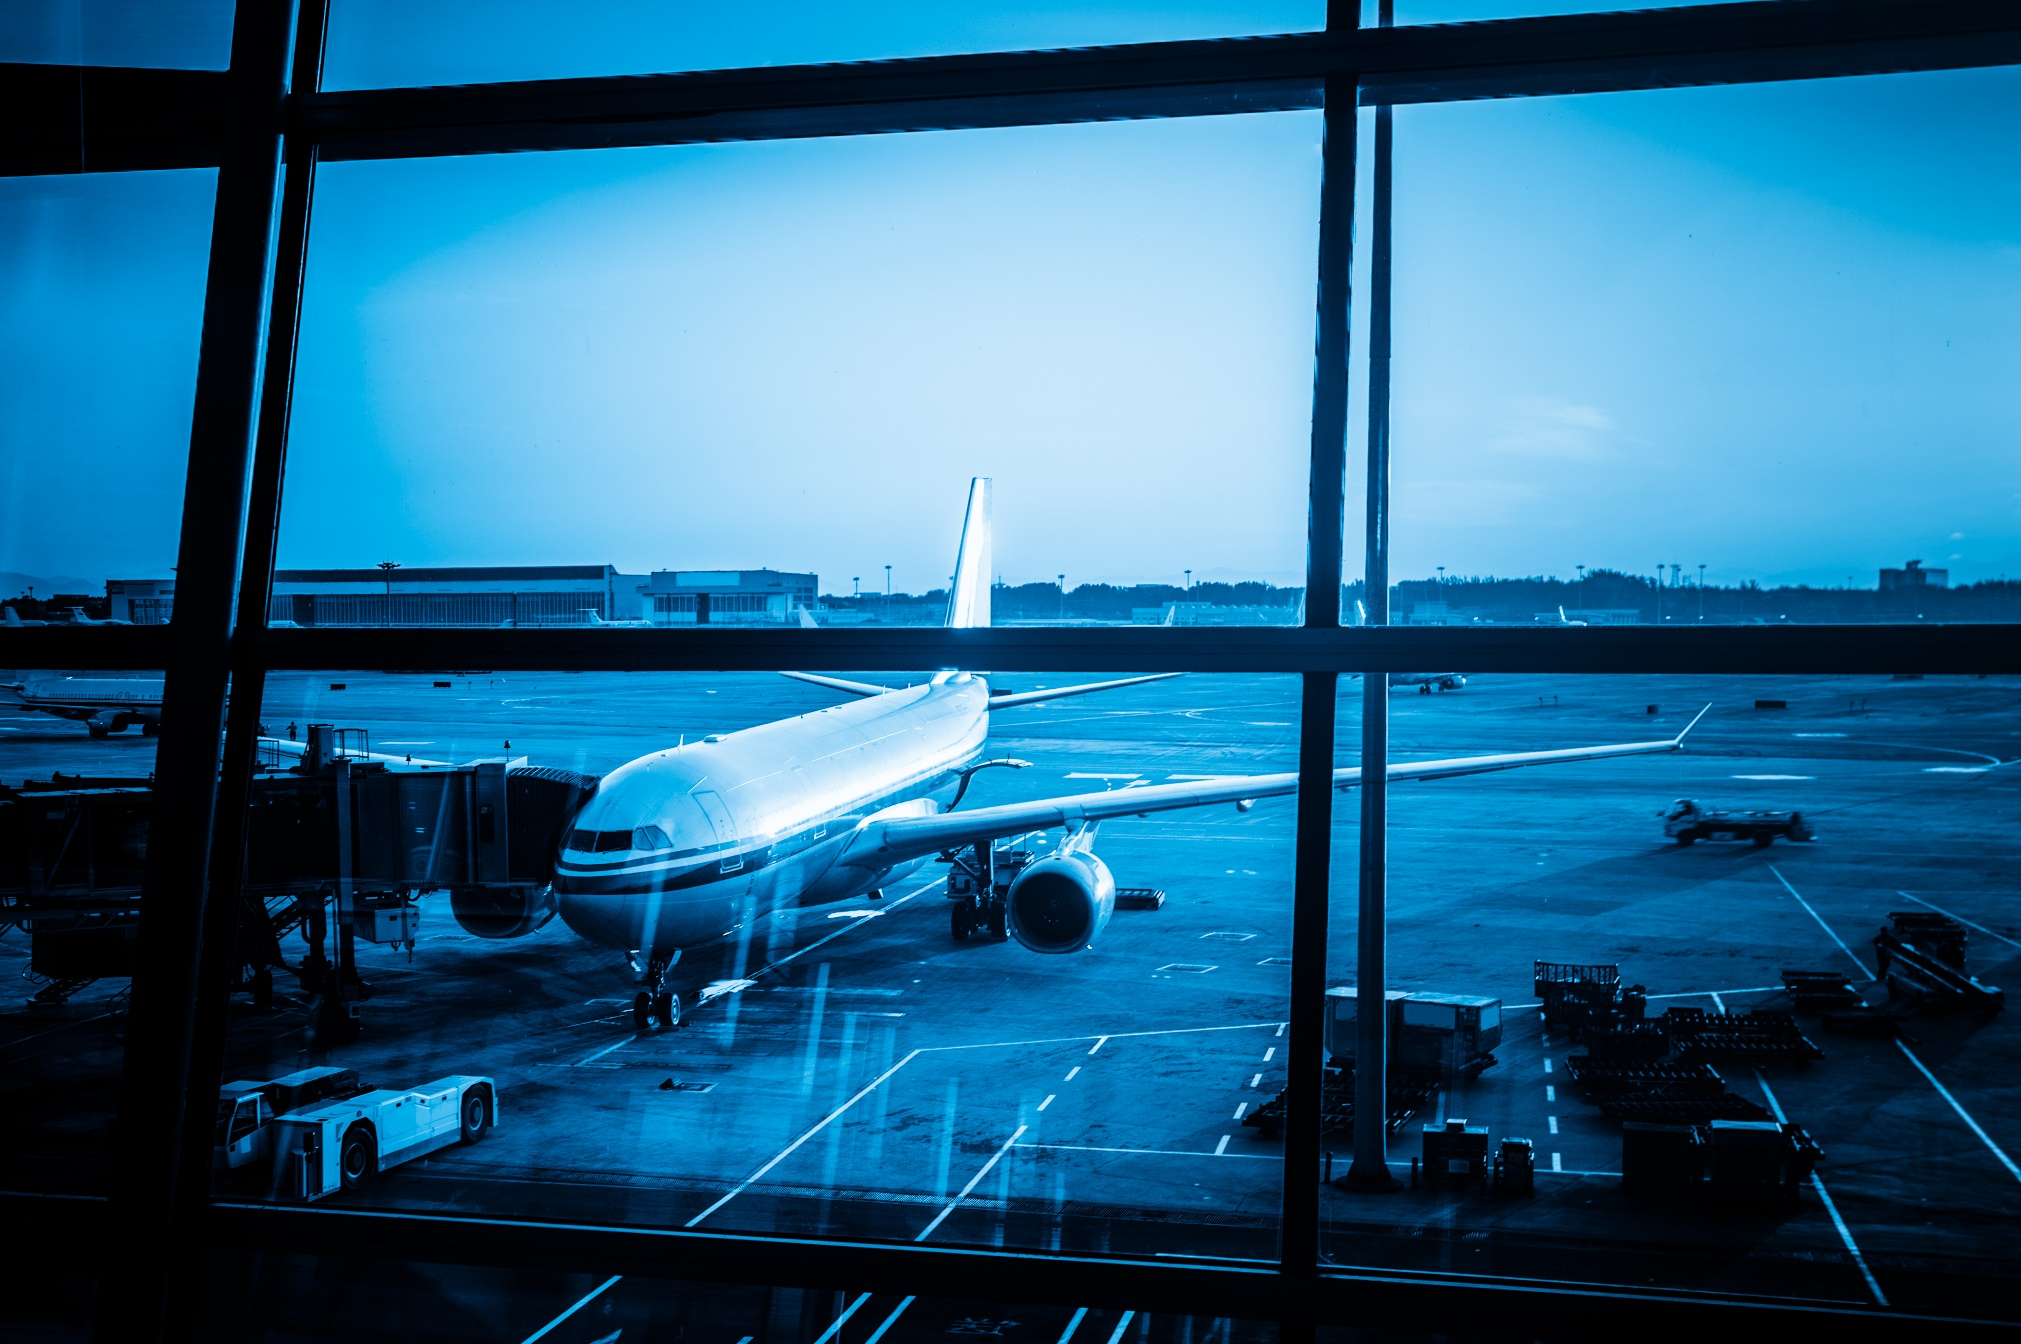
\includegraphics[width=\paperwidth, height=14.5cm]{plane.jpg}};
		\node[rectangle, fill=mygreen, anchor=north west, minimum width=20.5cm, minimum height=5.75cm,outer sep=0] (B) at ([xshift=-1pt,yshift=3.25cm]A.south west) {};
		\node[anchor=south] at ([yshift=7mm]A.north){
\includegraphics[width=7.18cm]{logo.png}};
		\node[rectangle, anchor=north west, text=white, align=left] (C) at ([xshift=10mm, yshift=2.75cm]A.south west) {
		{\fontsize{50}{60}\selectfont ENVISA} \\[9mm]
		{\fontsize{34}{42}\selectfont\bfseries AVIATION \& ENVIRONMENTAL}\\[7mm]
		{\fontsize{34}{42}\selectfont\bfseries SOLUTIONS }
		};
		\node[anchor=north west, align=left, font=\bfseries] at ([xshift=10.53mm, yshift=-0.48cm]B.south west) {62 rue Montorgueil \\ BAL 9\\ 75002 Paris \\ FRANCE \\ \url{www.env-isa.com} };
		\node[anchor=north east, align=right, font=\LARGE\bfseries] at ([xshift=1mm, yshift=-0.2cm]B.south east) {\airport \\[5pt] \report \\[5pt] \monthyear};
		\end{tikzpicture}
	\end{titlepage}
	% credits page
	\thispagestyle{empty}
	\begin{tikzpicture}[remember picture,overlay]
	\node[anchor=south west] at ([xshift=1.9cm,yshift=1in]current page.south west) {
\includegraphics[width=4.33cm]{riyadh.png}};
	\node[anchor=south east, align=right] (A) at ([xshift=-1.9cm,yshift=1.09in]current page.south east) {E-mail: \href{mailto:gabriel.casas@env-isa.com}{gabriel.casas@env-isa.com}\\\href{mailto:michele.cremaschi@env-isa.com}{ben.romarowski@env-isa.com}};	
	\node[anchor=south east,font=\bfseries, align=right] (B) at ([yshift=12pt]A.north east) {Gabriel Casas \\ Ben Romarowski};
	\node[anchor=south east,font=\bfseries, align=right] at ([yshift=12pt]B.north east) {Dated on: \\ \datedon};
	\end{tikzpicture}

\tableofcontents
\listoffigures
\begingroup
\let\clearpage\relax
\vspace*{3cm}
\listoftables
\endgroup

\addtocontents{toc}{\protect\addvspace{20pt}}
\addtocontents{lof}{\protect\addvspace{20pt}}
\addtocontents{lot}{\protect\addvspace{20pt}}

\chapter{Introduction}

In this report, the air pollutant levels, noise and meteorological measurements, as well as the traffic information are provided for the study period of \monthyear \ for Riyadh Airport.

The sensors network and the measured variables are described, followed by the meteorological measurements registered during the above-mentioned study period. In addition, the following emissions measurements are included per sensor: \ce{CO}, \ce{NO2}, \ce{O3}, \ce{SO2}, $\text{PM}_{2.5}$, \ce{PM10}, \ce{PM1}, \ce{CO2}, \ce{H2S}, \ce{NO} as well as the noise metrics: Leq, Lmin and Lmax. 

There is as well a section about traffic, which shows the time distribution of aircraft movements as well as the use of the terminals and runways.

With the previously gathered information, an analysis of the measurements is included, in which the influence of weather parameters and air traffic on the pollutant levels is commented. In order to perform this reasoning, events with high pollutant levels are analysed together with the traffic and the wind characteristics of that event.

At the final part of the report, a section about the USEPA Air Quality Standards and the related Air Quality Index is also included. This metric allows a general analysis of the air quality of the study area. Right after this section, the conclusions of the report can be found.

All the emission measurements, traffic distribution, temperature and humidity data can be found in the Appendixes, at the end of this document. This report also includes in this annex charts that show the sensors pollutants measurements grouped together for the study period.

\emptystations 	




\chapter{Sensors information}

\stationsnbr\ sensors with the objective of monitoring the air quality were installed at Riyadh Airport. Each of them provides measurements regarding Air Quality as well as meteorological information. The list of devices with their coordinates and measured variables is shown in Table~\ref{table:listsensors} and Table~\ref{table:listsensors2}.

\begin{table}[htb]
\caption{List of sensors (1)}\label{table:listsensors}
\small
\begin{tabular}{|>{\centering\arraybackslash}m{1cm}|>{\centering\arraybackslash}m{2.15cm}|>{\centering\arraybackslash}m{1.9cm}|>{\centering\arraybackslash}m{2cm}|>{\centering\arraybackslash}m{1.85cm}|m{6.1cm}|}\hline
\bfseries Label &\bfseries Device ID &\bfseries \breakcell{Device \\[-2pt] Name} &\bfseries Latitude &\bfseries Longitude & \centering\arraybackslash\bfseries Measured variables \\\hline
1 & SEN01P0001 & \breakcell[c]{Privet\\Aviation} & 24.965448 & 46.722919 & $\text{PM}_{2.5}$, \ce{PM10}, \ce{PM1}, \ce{CO2}, Temperature, Humidity, Light, UV, Leq, Lmax, Lmin, \ce{SO2}, \ce{CO}, \ce{H2S}, \ce{NO}, \ce{NO2}, \ce{O3}, Wind direction, Wind speed \\\hline
2 & SEN01P0002 & Primary Runway & 24.963136 & 46.712787 & \ce{PM_{2.5}}, \ce{PM10}, \ce{PM1}, \ce{CO2}, Light, UV, Leq, Lmax, Lmin, \ce{CO}, \ce{SO2}, \ce{O3}, \ce{NO}, \ce{NO2}, \ce{H2S}. \\\hline
3 & SEN01P0003 & ATC Tower & 24.9560084 & 46.697312 & \ce{PM_{2.5}}, \ce{PM10}, \ce{PM1}, \ce{CO2}, Light, UV, Leq, Lmax, Lmin, \ce{CO}, \ce{SO2}, \ce{O3}, \ce{NO}, \ce{NO2}, \ce{H2S}. \\\hline
4 & SEN01P0004 & \breakcell[c]{Royal\\Terminal} & 24.95376 & 46.695125 & \ce{PM_{2.5}}, \ce{PM10}, \ce{PM1}, \ce{CO2}, Temperature, Humidity, Light, UV, Leq, Lmax, Lmin, \ce{CO}, \ce{SO2}, \ce{O3}, \ce{NO}, \ce{NO2}, \ce{H2S} \\\hline
5 & SEN01P0005 & Air Cargo & 24.976318 & 46.694 & \ce{PM_{2.5}}, \ce{PM10}, \ce{PM1}, \ce{CO2}, Temperature, Humidity, Light, UV, Leq, Lmax, Lmin, \ce{SO2}, \ce{O3}, \ce{CO}, \ce{NO}, \ce{NO2}, \ce{H2S} \\\hline
6 & SEN01P0006 & Secondary Runway 01 & 24.956003 & 46.682273 & \ce{PM_{2.5}}, \ce{PM10}, \ce{PM1}, Light, UV, Leq, Lmax, Lmin, \ce{SO2}, \ce{NO2}, \ce{O3}, \ce{CO}, \ce{NO}, \ce{H2S} \\\hline
7 & SEN01P0007 & Secondary Runway 02 & 24.941005 & 46.691696 & \ce{PM_{2.5}}, \ce{PM10}, \ce{PM1}, \ce{CO2}, Temperature, Humidity, Light, UV, Leq, Lmax, Lmin, \ce{SO2}, \ce{NO2}, \ce{O3}, \ce{CO}, \ce{NO}, \ce{H2S} \\\hline
8 & SEN01P0008 & Fire Station & 24.963901 & 46.685287 & \ce{PM_{2.5}}, \ce{PM10}, \ce{PM1}, \ce{CO2}, Temperature, Humidity, Light, UV, Leq, Lmax, Lmin, \ce{SO2}, \ce{NO2}, \ce{O3}, \ce{CO}, \ce{NO}, \ce{H2S} \\\hline

\end{tabular}
\end{table}
\begin{table}
\caption{List of sensors (2)}\label{table:listsensors2}
\small
\begin{tabular}{|>{\centering\arraybackslash}m{1cm}|>{\centering\arraybackslash}m{2.15cm}|>{\centering\arraybackslash}m{1.9cm}|>{\centering\arraybackslash}m{2cm}|>{\centering\arraybackslash}m{1.85cm}|m{6.1cm}|}\hline
\bfseries Label &\bfseries Device ID &\bfseries \breakcell{Device \\[-2pt] Name} &\bfseries Latitude &\bfseries Longitude & \centering\arraybackslash\bfseries Measured variables \\\hline
9 & SEN02P0003 & CS 59 Storage & 24.938702 & 46.739647 & \ce{PM_{2.5}}, \ce{PM10}, \ce{CO2}, Temperature, Humidity, Light, UV, Leq, Lmax, Lmin, \ce{SO2}, \ce{NO2}, \ce{O3}, \ce{CO}, \ce{NO}, \ce{NO2}, \ce{H2S} \\\hline
10 & SEN02P0002 & AE123 Inbound K.S.R & 24.854928 & 46.681631 & \ce{PM_{2.5}}, \ce{PM10}, \ce{CO2}, Temperature, Humidity, Light, UV, Leq, Lmax, Lmin, \ce{SO2}, \ce{NO2}, \ce{O3}, \ce{CO}, \ce{NO}, \ce{NO2}, \ce{H2S} \\\hline
11 & SEN02P0001 & Family Camp & 24.941528 & 46.649335 & \ce{PM_{2.5}}, \ce{PM10}, \ce{CO2}, Temperature, Humidity, Light, UV, Leq, Lmax, Lmin, \ce{SO2}, \ce{NO2}, \ce{O3}, \ce{CO}, \ce{NO}, \ce{NO2}, \ce{H2S} \\\hline
12 & SEN02P0005 & SASCO Station 3 & 24.890091 & 46.693224 & \ce{PM_{2.5}}, \ce{PM10}, \ce{CO2}, Temperature, Humidity, Light, UV, Leq, Lmax, Lmin, \ce{SO2}, \ce{NO2}, \ce{O3}, \ce{CO}, \ce{NO}, \ce{NO2}, \ce{H2S} \\\hline
13 & SEN02P0004 & RIYADH FRONT (SASCO STATION 1) & 24.844891 & 46.732690 & \ce{PM_{2.5}}, \ce{PM10}, \ce{CO2}, Temperature, Humidity, Light, UV, Leq, Lmax, Lmin, \ce{SO2}, \ce{NO2}, \ce{O3}, \ce{CO}, \ce{NO}, \ce{NO2}, \ce{H2S}
 \\\hline
\end{tabular}
\end{table}


The second table shows the new stations installed in 2021. In addition, satellite images with the
locations of the sensors can be found below in Figures 1 and 2.

\IfFileExists{map1.png}
{\begin{figure}[H]
\centering
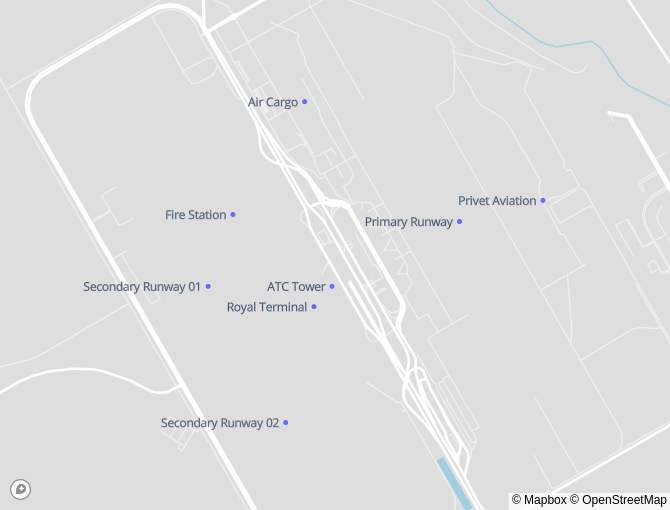
\includegraphics[width=0.7\textwidth, keepaspectratio]{map1.png}
\caption{Location of the sensors (1)}\label{image4}
\end{figure}}

\IfFileExists{map2.png}
{\begin{figure}[H]
\centering
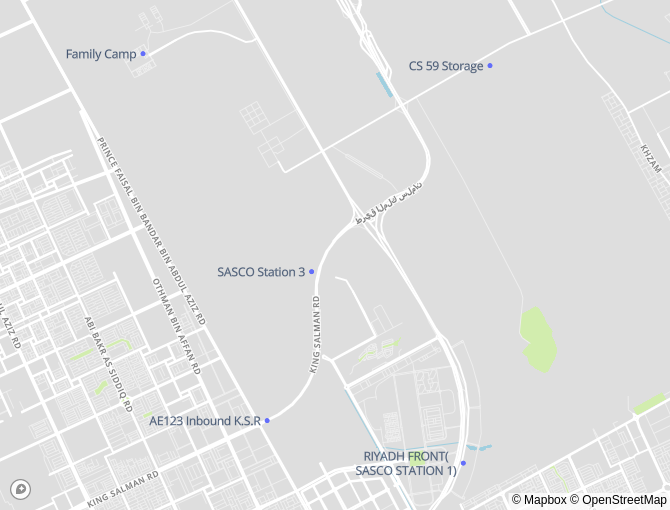
\includegraphics[width=0.7\textwidth, keepaspectratio]{map2.png}
\caption{Location of the sensors (2)}\label{image4}
\end{figure}}

\chapter{Meteorological measurements}


\section{Wind roses}

The average wind rose for the last 5 years\footnote{Historical wind data obtained from the General Authority for Statistics via KAPSARC dataportal} as well as the one referring to  \monthyear \ are presented. From the wind roses can be observed that the most predominant winds are the ones from South East and North directions, having usually the latter ones the highest speeds. In the case of \monthyear , \ there was a predominance of \freqWinds\ winds. The highest speeds were mostly registered from \maxWind .

\IfFileExists{windrosemonth.png}
{\begin{figure}[H]
\begin{minipage}[b]{0.5\textwidth}
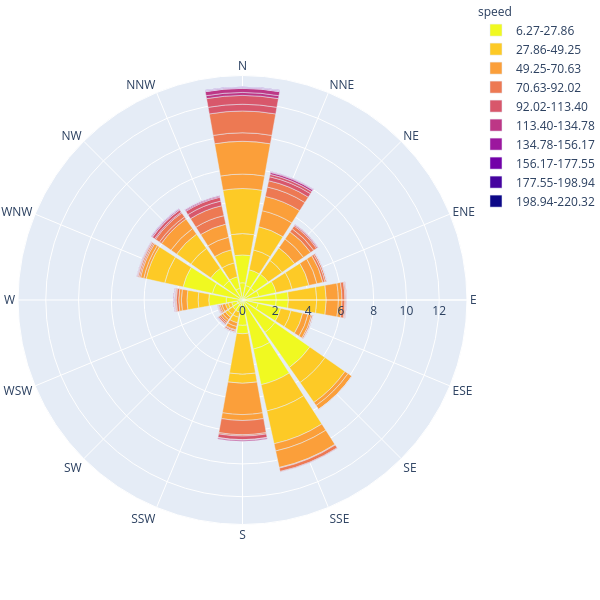
\includegraphics[width=\textwidth]{windrose5yrs}
\caption{Average Wind rose last 5 years}\label{windrose10years}
\end{minipage}
\begin{minipage}[b]{0.5\textwidth}
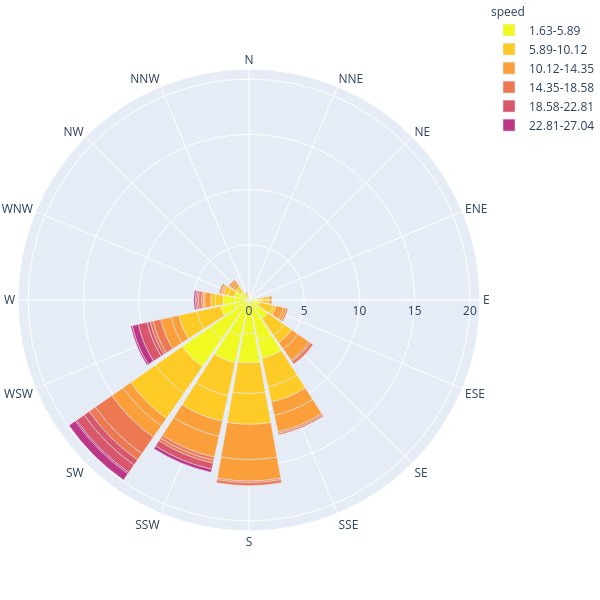
\includegraphics[width=\textwidth]{windrosemonth}\label{windrosemonth}
\caption{\monthyear \ Wind rose}
\end{minipage}
\end{figure}}

\section{Temperature}

See Appendixes, Figure A-1

\section{Humidity}
 
See Appendixes, Figure A-2

\chapter{Emissions measurements}

All the graphs related to the emissions measurements are presented in Appendixes, Figure A-3 to A-106. 

\chapter{Noise measurements}

In this section, the average values of the 3 available noise metrics (Leq, Lmin and Lmax) are shown for the study period for each of the stations. The highest Leq values were obtained in the \maxNoise\ station, while the lowest corresponded to the \minNoise.

\section{Leq}

\IfFileExists{image1.png}
{\begin{figure}[H]
\centering
\qquad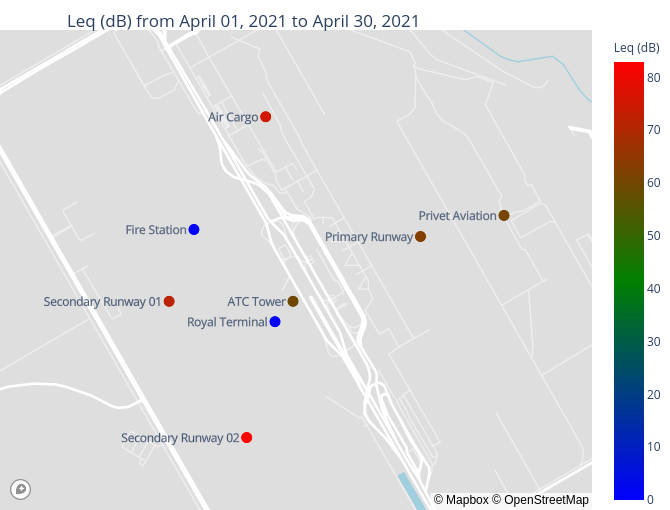
\includegraphics[width=0.7\textwidth, keepaspectratio]{image1}
\caption{Average Leq (dB) per station for \monthyear (1)}\label{image1}
\end{figure}}{}

\IfFileExists{image4.png}
{\begin{figure}[H]
\centering
\qquad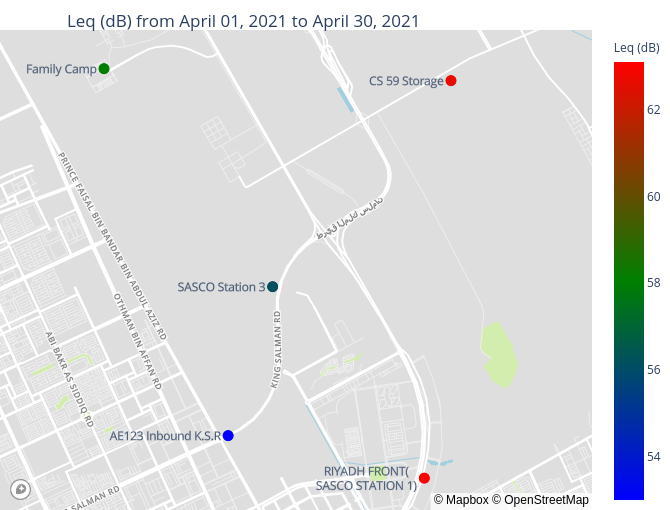
\includegraphics[width=0.7\textwidth, keepaspectratio]{image4}
\caption{Average Leq (dB) per station for \monthyear (2)}\label{image4}
\end{figure}}{}


\section{Lmin}

\IfFileExists{image2.png}
{\begin{figure}[H]
\centering
\qquad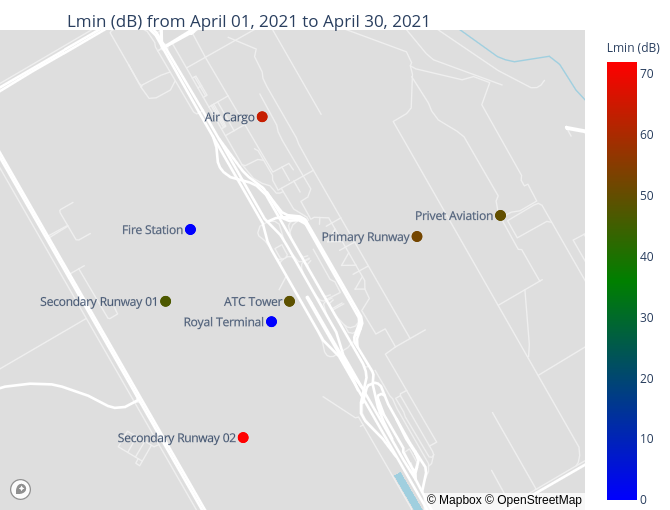
\includegraphics[width=0.7\textwidth, keepaspectratio]{image2}
\caption{Average Lmin (dB) per station for \monthyear (1)}\label{image2}
\end{figure}}{}

\IfFileExists{image5.png}
{\begin{figure}[H]
\centering
\qquad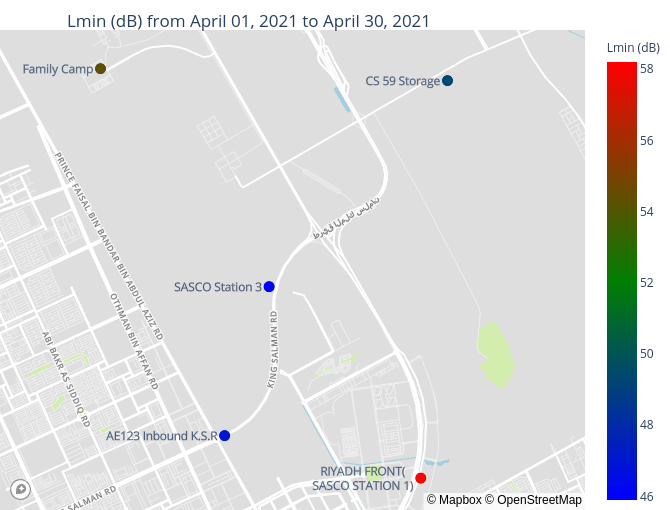
\includegraphics[width=0.7\textwidth, keepaspectratio]{image5}
\caption{Average Lmin (dB) per station for \monthyear (2)}\label{image5}
\end{figure}}{}

\section{Lmax}

\IfFileExists{image3.png}
{\begin{figure}[H]
\centering
\qquad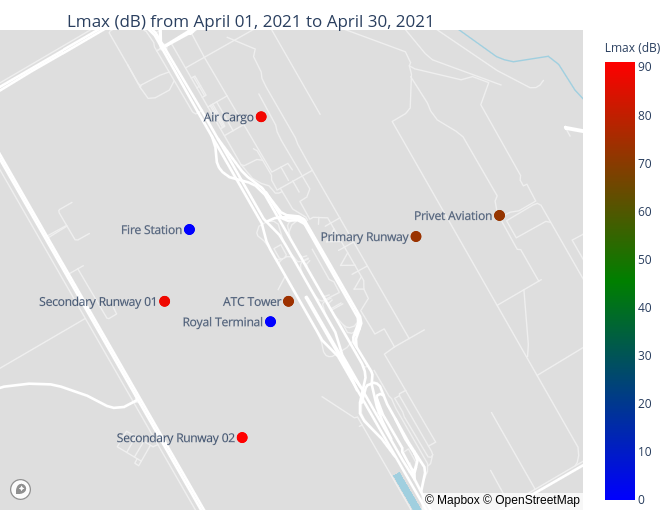
\includegraphics[width=0.7\textwidth, keepaspectratio]{image3}
\caption{Average Lmax (dB) per station for \monthyear (1)}\label{image3}
\end{figure}}{}

\IfFileExists{image6.png}
{\begin{figure}[H]
\centering
\qquad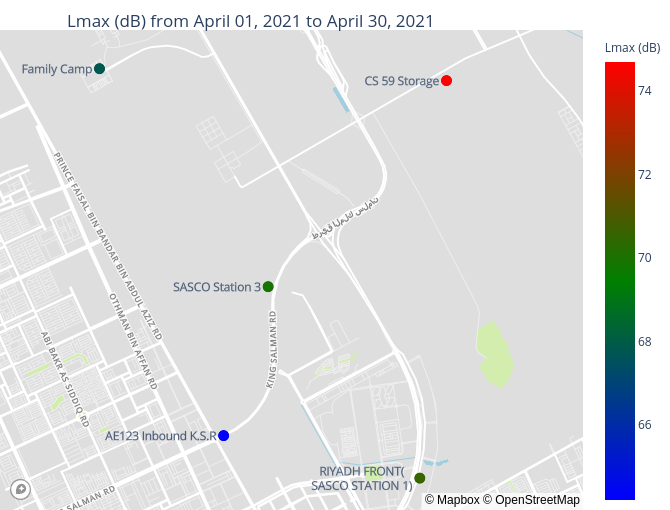
\includegraphics[width=0.7\textwidth, keepaspectratio]{image6}
\caption{Average Lmax (dB) per station for \monthyear (2)}\label{image6}
\end{figure}}{}



\chapter{Traffic information}

The highest number of flights took place on average  \trafficPeriod \ (with a peak at \trafficHour) and on \trafficDay . Compared to the previous month, the number of flights show a \trafficChange. The traffic temporal distribution chart can be consulted in the Appendixes.


\IfFileExists{image7.png}
{\begin{figure}[H]
\centering
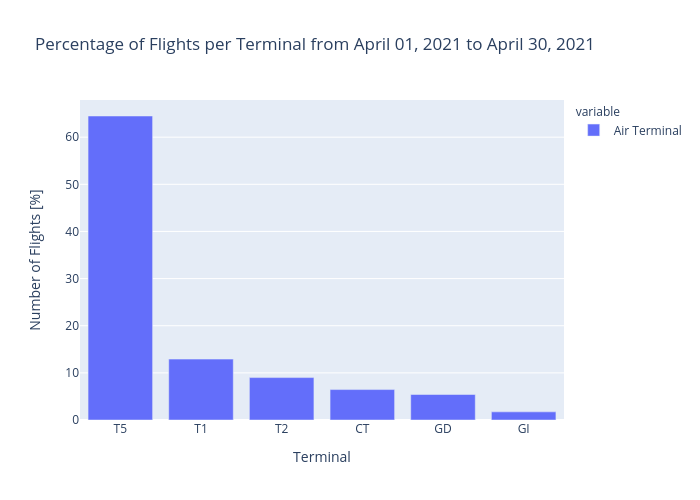
\includegraphics[width=0.75\textwidth, keepaspectratio]{image7}
\caption{Terminal use percentage}\label{image7}
\end{figure}}{}


The major part of flights are linked to Terminal \maxTerminal . Terminal 5 handles domestic flights and is situated at the south side of the airport. The Terminals 1 and 2 are used for international flights.

%Concerning the distribution of the traffic among terminal, more than 50\% of the flights were linked to the Terminal T5. 

\IfFileExists{image8.png}
{\begin{figure}[H]
\centering
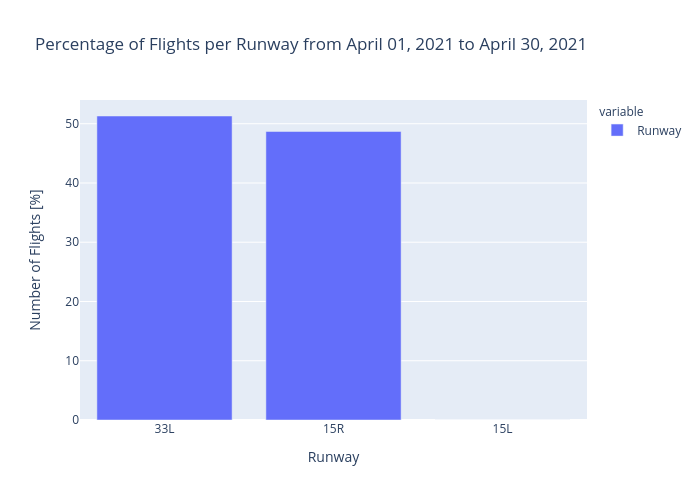
\includegraphics[width=0.75\textwidth, keepaspectratio]{image8}
\caption{Runway use percentage}\label{image8}
\end{figure}}{}

Most of the traffic was allocated to runway in direction \maxRunway.

\IfFileExists{image9.png}
{\begin{figure}[H]
\centering
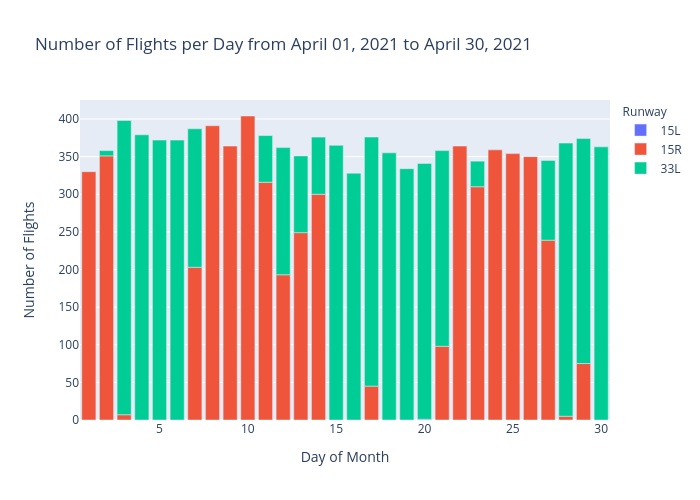
\includegraphics[width=0.75\textwidth, keepaspectratio]{image9}
\caption{Number of flights per day and per runway}\label{image9}
\end{figure}}{}

The previous chart shows the distribution of flights among the runways during the studied period. 


\chapter{Analysis of measurements}

In this section, the measurements obtained are commented together with the traffic and weather data. 

\section{CO}

The recorded \ce{CO} levels were found to \tresholdCO\ the considered USEPA treshold (\limitCO $mg/m^3$).

%The \ce{CO} values registered by the different sensors are broadly comparable and are below the considered \ce{CO} USEPA limit, which is 35 ppm. For all the stations, the values fall in the range between 0 and 3 mg/m\textsuperscript{3} and no significant differences are found among the sensors. 

Regarding the temporal distribution, the CO levels show a average minimum \minDailyCO\ and average maximum \maxDailyCO .

From a monthly perspective, the average CO levels experienced a \monthChangeCO\ in comparison with the previous month average.


\IfFileExists{image10.png}
{\begin{figure}[H]
\centering
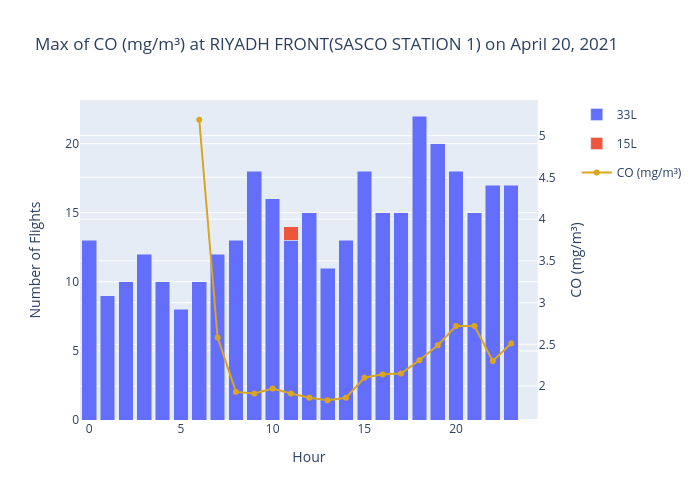
\includegraphics[width=0.95\textwidth, keepaspectratio]{image10}
\caption{Traffic and \ce{CO} peak level}\label{image10}
\end{figure}}{}

A \ce{CO} peak was found on \dayMaxCO \ at the station \stationMaxCO . %This peak \relTrafficMaxCO . 
Furthermore, the Pearson coefficient of correlation for these two variables during the day of maximum ocurrance is \correlCO .  

\IfFileExists{windroseCO.png}
{\begin{figure}[H]
\centering
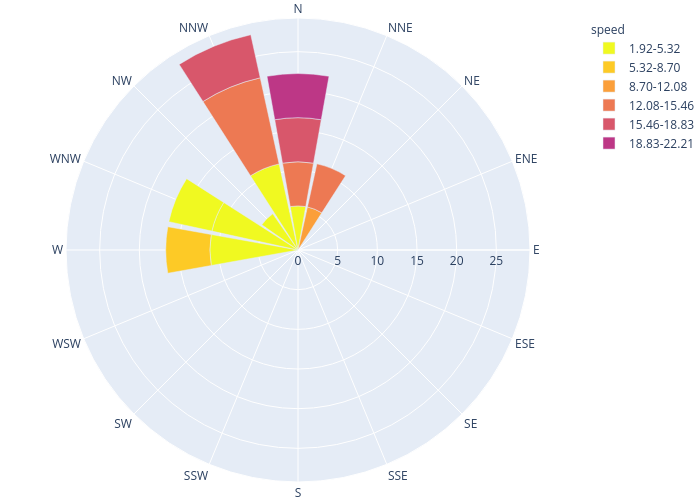
\includegraphics[width=.8\textwidth, keepaspectratio]{windroseCO}
\caption{Windrose CO peak level}\label{windroseCO}
\end{figure}}{}

The wind rose for this day shows that the \windCO

\section{\ce{NO2}}

The registered \ce{NO_2} levels were found to \tresholdNOtwo\ the considered USEPA treshold (\limitNOtwo $\mu g/m^3$).

The highest average \ce{NO_2} levels was found \maxDailyNOtwo\ whereas the minimum was found \minDailyNOtwo.

The monthly average values experienced a \monthChangeNOtwo in comparison with the previous month.


The highest measurement of the studied period was registered on  \dayMaxNOtwo , at the station \stationMaxNOtwo.

\IfFileExists{image11.png}
{\begin{figure}[H]
\centering
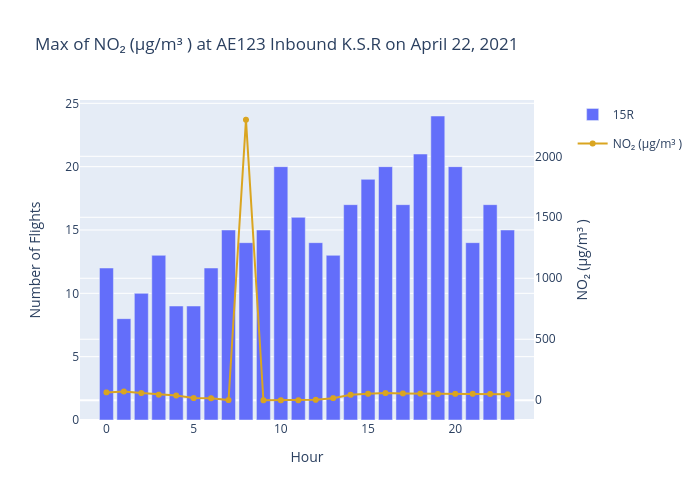
\includegraphics[width=0.98\textwidth]{image11}
\caption{Traffic and \ce{NO2} peak level}\label{image11}
\end{figure}}{}

%As it can be seen in the previous chart, the highest value \relTrafficMaxNOtwo.
Furthermore, the Pearson coefficient of correlation for these two variables during the day of maximum ocurrance is \correlOthree .  

\IfFileExists{windroseNO₂.png}
{\begin{figure}[H]
\centering
	\includegraphics[width=0.8\textwidth, keepaspectratio]{windroseNO₂}
\caption{Windrose \ce{NO2} peak level}\label{windroseNO2}
\end{figure}}{}

For this date, the \windNOtwo


\section{\ce{O3}}

The recorded \ce{O_3} levels were found to \tresholdOthree\ the considered USEPA treshold (\limitOthree $\mu g/m^3$).

The highest average \ce{O_3} levels was found \maxDailyOthree\ whereas the minimum was found \minDailyOthree.

%Daily fluctuations were observed in the concentration levels registered by the sensors.

The monthly average values experienced a \monthChangeOthree in comparison with the previous month.

%ASK GABI
These daily levels were found to have an anti-correlated behaviour (peaks of O3 when NO2 levels were low and vice versa) in relation to NO2, related to the photochemical processes associated with NOx.

\IfFileExists{image12.png}
{\begin{figure}[H]
\centering
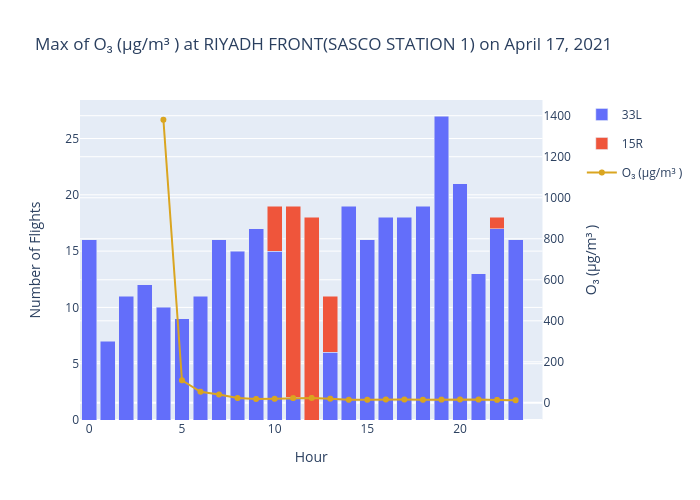
\includegraphics[width=0.98\textwidth, keepaspectratio]{image12}
\caption{Traffic and \ce{O3} peak level}\label{image12}
\end{figure}}{}


The highest measurement of the studied period was registered  on \dayMaxOthree \ at the station \stationMaxOthree . 
%This peak \relTrafficMaxOthree . 
Furthermore, the Pearson coefficient of correlation for these two variables during the day of maximum ocurrance is \correlOthree .  

\IfFileExists{windroseO₃.png}
{\begin{figure}[H]
\centering
\includegraphics[width=0.8\textwidth, keepaspectratio]{windroseO₃}
\caption{Windrose \ce{O3} peak level}\label{windroseO3}
\end{figure}}{}

For this date, the \windOthree


\section{\ce{SO2}}

The recorded SO2 levels were found to \tresholdSOtwo\ the considered USEPA threshold (\limitSOtwo $\mu g/m^3$) and the highest levels occurred usually during the evening.

The highest average \ce{SO_2} levels was found \maxDailySOtwo\ whereas the minimum was found \minDailySOtwo .

In the case of this pollutant, the average concentrations experienced a \monthChangeSOtwo in comparison with the levels obtained during the previous month.

The highest measurement of the studied period was registered  on \dayMaxSOtwo \ at the station \stationMaxSOtwo . 
%This peak \relTrafficMaxSOtwo .
Furthermore, the Pearson coefficient of correlation for these two variables during the day of maximum ocurrance is \correlSOtwo .  

\IfFileExists{image13.png}
{\begin{figure}[H]
\centering
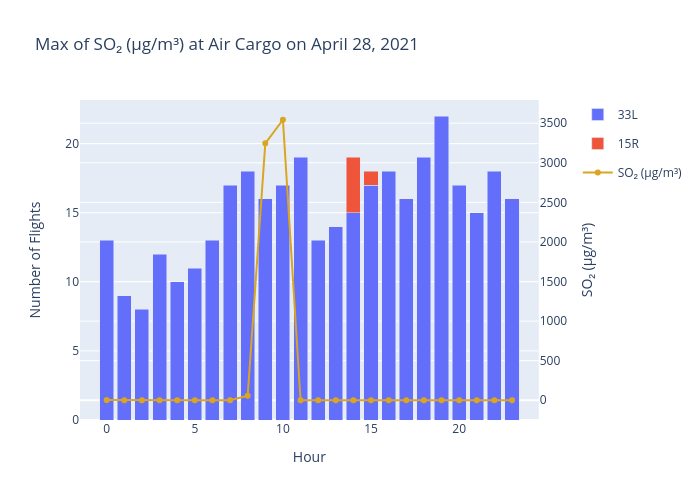
\includegraphics[width=0.98\textwidth,keepaspectratio]{image13}
\caption{Traffic and \ce{SO2} levels}\label{image13}
\end{figure}}{}

For this date, the \windSOtwo

\IfFileExists{windroseSO₂.png}
{\begin{figure}[H]
\centering
	\includegraphics[width=0.8\textwidth, keepaspectratio]{windroseSO₂}
\caption{Windrose \ce{SO2} peak level}\label{windroseSO2}
\end{figure}}{}


\section{Particulate matter}

The recorded \ce{PM_{2.5}} levels were found to \tresholdPMtwofive\ the considered USEPA treshold (35 $\mu g/m^3$).



%The PM values stayed below the respective USEPA threshold during the studied month and showed in most of the stations slighthly lower values to the ones obtained during the previous months.

The monthly average values of \ce{PM_{2.5}} experienced a \monthChangePMtwofive in comparison with the previous month.

The highest average \ce{PM_{2.5}} levels was found \maxDailyPMtwofive\ whereas the minimum was found \minDailyPMtwofive .

The highest \ce{PM_{2.5}} values of the month were obtained during  \dayMaxPMtwofive \ at the station \stationMaxPMtwofive . 
%This peak \relTrafficMaxPMtwofive .
Furthermore, the Pearson coefficient of correlation for these two variables during the day of maximum ocurrance is \correlPMtwofive .  The registered levels as well as the traffic for that date are shown in the Figure below.

\IfFileExists{image14.png}
{\begin{figure}[H]
\centering
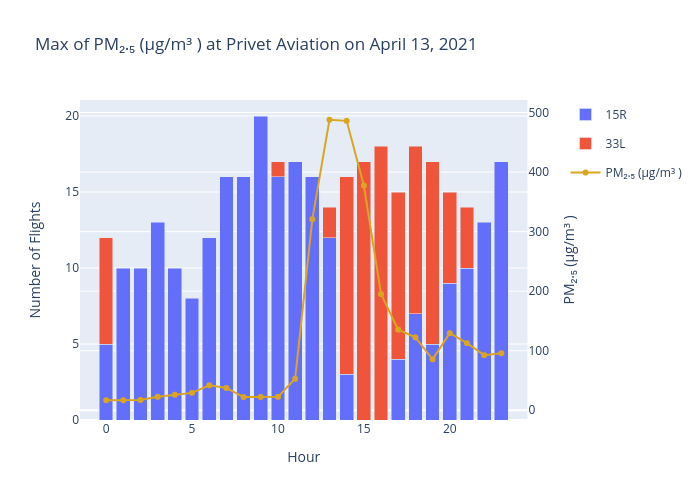
\includegraphics[width=0.95\textwidth, keepaspectratio]{image14}
\caption{Traffic and \ce{PM_{2.5}} peak level}\label{image14}
\end{figure}}{}



In the case of the \ce{PM10}, the highest levels were measured at the \stationMaxPMten\ sensor on \dayMaxPMten . 
%This peak \relTrafficMaxPMten .  
Furthermore, the Pearson coefficient of correlation for these two variables during the day of maximum ocurrance is \correlPMten .

The monthly average values of \ce{PM10} experienced a \monthChangePMten in comparison with the previous month.


Considering the levels of \ce{PM_{10}} recorded, they were found to \tresholdPMten\ the considered USEPA treshold (150 $\mu g/m^3$).

The highest average \ce{PM10} levels was found \maxDailyPMten\ whereas the minimum was found \minDailyPMten .


\IfFileExists{image15.png}
{\begin{figure}[H]
\centering
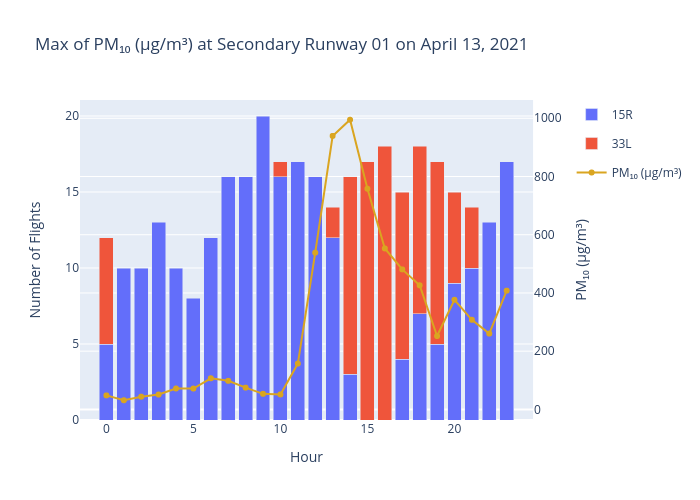
\includegraphics[width=0.95\textwidth, keepaspectratio]{image15}
\caption{Traffic and \ce{PM10} peak level}\label{image15}
\end{figure}}{}


\IfFileExists{windrosePM₁₀.png}
{\begin{figure}[H]
\centering
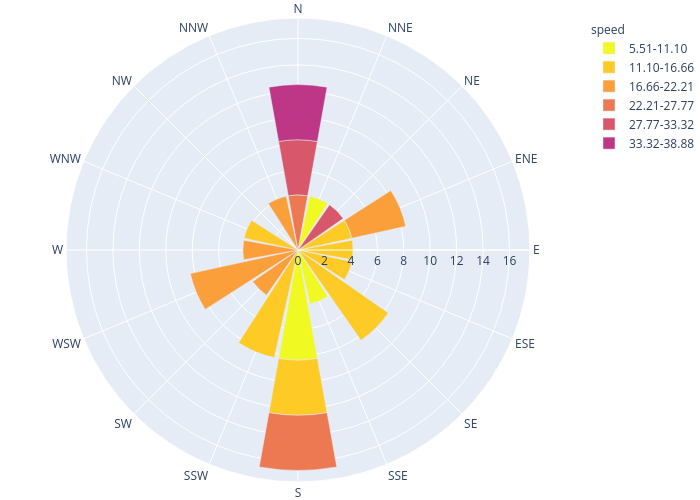
\includegraphics[width=0.8\textwidth, keepaspectratio]{windrosePM₁₀}
\caption{Windrose PM peak level}\label{windrosePM10}
\end{figure}}{}

On this day, the \windPMten

\section{\ce{H2S}}


%The daily fluctuation of the H2S values follows a similar trend along the stations. The values decrease slowly during the night and early morning hours, increasing afterwards along the day. The highest peaks are found during the late evening, decreasing afterwards.

The highest average \ce{H2S} level was found \maxDailyHtwoS\ whereas the minimum was found \minDailyHtwoS .


In the case of this pollutant, the average concentrations experienced a \monthChangeHtwoS in comparison with the levels obtained during the previous month.


The \ce{H2S} maximum level was recorded at the station \stationMaxHtwoS, on \dayMaxHtwoS . 
%This peak \relTrafficMaxPMten .  
Furthermore, the Pearson coefficient of correlation for these two variables during the day of maximum ocurrance is \correlHtwoS .

The registered concentrations, as well as the air traffic movements from that date are represented in the following figure:

\IfFileExists{image17.png}
{\begin{figure}[H]
\centering
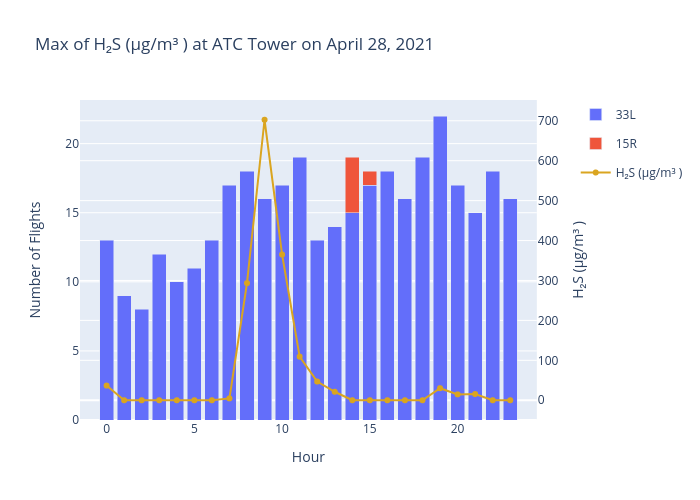
\includegraphics[width=0.95\textwidth, keepaspectratio]{image17}
\caption{Traffic and \ce{H2S} peak level}\label{image17}
\end{figure}}{}

On this date, the \windHtwoS

\IfFileExists{windroseH₂S.png}
{\begin{figure}[H]
\centering
\includegraphics[width=0.8\textwidth, keepaspectratio]{windroseH₂S}
\caption{Windrose \ce{H2S} peak level}\label{windroseH2S}
\end{figure}}{}

\section{\ce{NO}}

%The NO levels show many fluctuations during the study period, with a clear daily pattern of low values during the morning and night and with a peak during the afternoon time. This pattern was found at all the stations, although the average peak concentrations were different among sensors. This daily fluctuation showed a negative correlation with the NO2 values, due to the conversion of NO2 into NO.

The NO levels show fluctuations during the study period, with a daily pattern with a minimum \minDailyNO\ a peak \maxDailyNO.

%ASK GABI about this
This daily fluctuation showed a negative correlation with the NO2 values, due to the conversion of NO2 into NO.

In the case of this pollutant, the average concentrations experienced a \monthChangeNO in comparison with the levels obtained during the previous month.


A particularly high peak of \ce{NO} levels was registered at the station \stationMaxNO\ on \dayMaxNO.

\IfFileExists{image18.png}
{\begin{figure}[H]
\centering
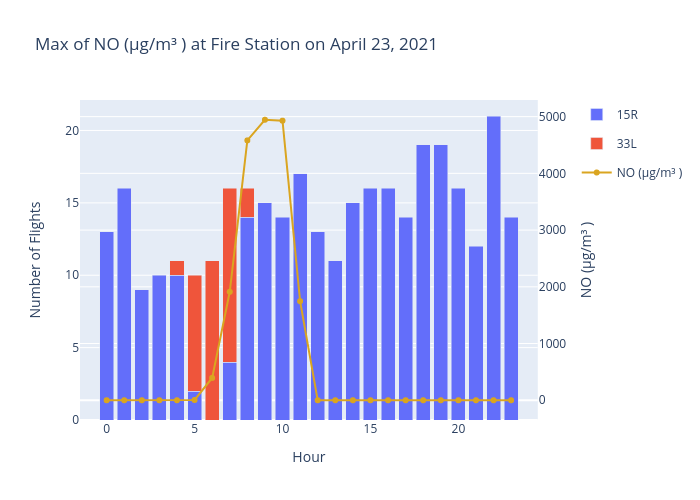
\includegraphics[width=0.95\textwidth, keepaspectratio]{image18}
\caption{Traffic and \ce{NO} peak level}\label{image18}
\end{figure}}{}

In the previous chart, the traffic at the runways as well as the NO levels are plotted for that station. 

\IfFileExists{windroseNO.png}
{\begin{figure}[H]
\centering
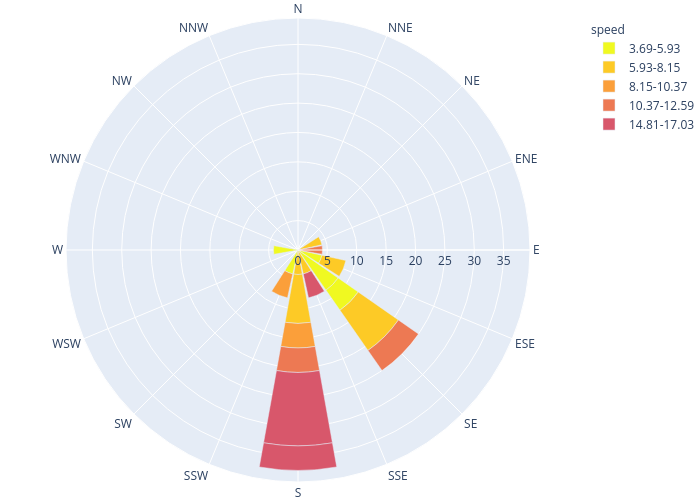
\includegraphics[width=0.8\textwidth, keepaspectratio]{windroseNO}
\caption{Windrose \ce{NO} peak level}\label{windroseNO}
\end{figure}}{}

The previous wind rose shows that the \windNO

%The maximum \relTrafficMaxNO .
Furthermore, the Pearson coefficient of correlation for these two variables during the day of maximum ocurrance is \correlNO .


\section{Noise}

As it can be seen in the noise measurement section, the highest levels are registered at the station \stationMaxLeq\ with maximum noise levels reaching \maxNoiseValue\ dB.

%In the case of noise, the average level experienced a \monthChangeLeq in comparison with the levels obtained during the previous month.

\IfFileExists{image21.png}
{\begin{figure}[H]
\centering
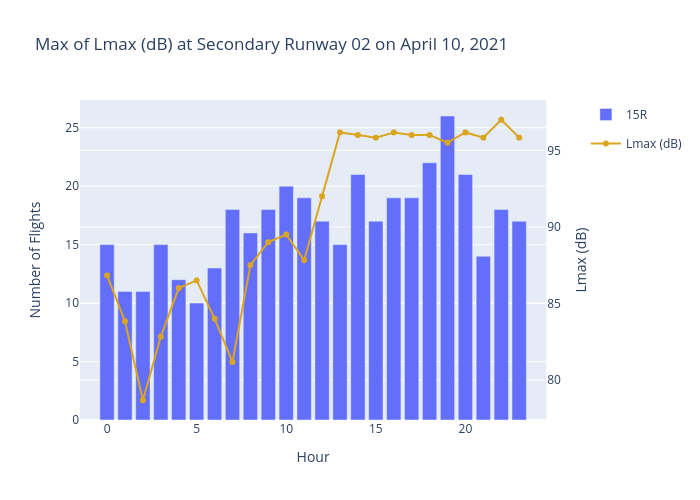
\includegraphics[width=0.98\textwidth]{image21}
\caption{Traffic and Lmax peak level}\label{image21}
\end{figure}}{}

%The maximum \relTrafficMaxLeq . 
Furthermore, the Pearson coefficient of correlation for these two variables during the day of maximum ocurrance is \correlLeq .

\chapter{Air Quality Standards and Air Quality Index (AQI)}

The United States Environmental Protection Agency (EPA) set \textbf{Air Quality Standards} for pollutants considered harmful to public health and the environment\footnote{NAAQS Table. EPA. \url{https://www.epa.gov/criteria-air-pollutants/naaqs-table}}. There are two types of standards. Primary standards are aimed to provide public health protection, including the protection of \textit{sensitive} groups like children and the elderly. The secondary standards have the goal to set public welfare protection, like protecting against decreased visibility and damage to animals, crops, vegetation and buildings.

From these standards, the following ones are considered in this study:

\begin{table}[H]
\centering
\small
\renewcommand\arraystretch{1.3}
\caption{Standards considered}\label{table:Standards}
\begin{tabular}{|>{\centering\arraybackslash\bfseries}m{1.9cm}|m{2.1cm}|m{1.85cm}|m{4cm}|}\hline
Pollutant &\centering\arraybackslash\bfseries Type &\centering\arraybackslash\bfseries Averaging time &\centering\arraybackslash \bfseries Level\footnotemark \\\hline
	\ce{CO} & Primary & 1 hour & 35 ppm $\left(\text{\limitCO}~mg/m^3\right)$ \\\hline
	\ce{NO2} & Primary & 1 hour & 100 ppb $\left(\text{\limitNOtwo}~\mu g/m^3\right)$ \\\hline
	\ce{SO2} & Primary & 1 hour & 75 ppb $\left(\text{\limitSOtwo}~\mu g/m^3\right)$ \\\hline
	\ce{O3} & Primary and secondary & 8 hours & 0.070 ppm $\left(\text{\limitOthree}~\mu g/m^3\right)$ \\\hline
\ce{PM_{2.5}} & Primary and secondary & 24 hours & 35 $\mu g/m^3$ \\\hline
\ce{PM10} & Primary and secondary & 24 hours & 150 $\mu g/m^3$ \\\hline
\end{tabular}
\end{table}

\footnotetext{Note: The units' conversions for the limits were calculated assuming the average temperature recorded during the month}

In addition, the \textbf{Air Quality Index developed by the US. Environmental Protection Agency}\footnote{Technical Assistance Document for the Reporting of Daily Air Quality Index (AQI) \url{https://www3.epa.gov/airnow/aqi-technical-assistance-document-sept2018.pdf}} has also been calculated with the pollutant concentrations obtained by the sensors. This index considers the concentrations of the previous pollutants (\ce{CO}, \ce{NO2}, \ce{SO2}, \ce{O3}, \ce{PM_{2.5}} and \ce{PM10}) in order to categorise the air quality into 6 different levels of health concern. Below, in Table~\ref{table:breakpoints}, the breakpoints for each pollutant and their respective categories are shown.

The purpose of the AQI is to visualize easily how the Air Quality of a certain location is. An AQI of 100 for a certain pollutant corresponds to its NAAQS levels. In our case, since we are obtaining information for several pollutants, the total AQI for a station corresponds to the largest AQI from the analysed levels. 

\begin{table}[H]
\centering
\small
\renewcommand\arraystretch{1.3}
\setlength{\tabcolsep}{4pt}
\caption{Concentration breakpoints, AQI and Category by pollutant}\label{table:breakpoints}
\resizebox{\textwidth}{!}{%
\begin{tabular}{*{8}{|c}|p{2.8cm}|}
\hline
\multicolumn{7}{|l|}{\bfseries Breakpoints}& & \\ \hline
\bfseries \breakcell{\ce{O3} \\[-6pt] (ppm) \\[-6pt] 8-hour} & \bfseries \breakcell{\ce{O3} \\[-6pt] (ppm)\\[-6pt] 1-hour} &\bfseries \breakcell{\ce{PM_{2.5}}\\[-4pt] \big(µg/m\textsuperscript{3}\big) \\[-5pt] 24-hour} & \bfseries \breakcell{\ce{PM10} \\[-4pt] \big(µg/m\textsuperscript{3}\big)\\[-5pt] 24-hour} & \bfseries \breakcell{\ce{CO}\\[-6pt] (ppm)\\[-6pt] 8-hour} & \bfseries \breakcell{\ce{SO2} \\[-6pt](ppb)\\[-6pt] 1-hour} & \bfseries \breakcell{\ce{NO2} \\[-6pt] (ppb)\\[-6pt] 1-hour} &\bfseries  AQI &\centering\arraybackslash\bfseries  Category \\ \hline
\rowcolor{good}0--0.054 &  & 0--12 & 0--54 & 0--4.4 & 0--35 & 0--53 & 0--50 & Good \rule[-0.9\baselineskip]{0pt}{2.2\baselineskip}\\ \hline
\rowcolor{moderate}0.055--0.070 &  & 12.1--35.4 & 55--154 & 4.5--9.4 & 36--75 & 54--100 & 51--100 & Moderate \rule[-0.9\baselineskip]{0pt}{2.2\baselineskip}\\ \hline
\rowcolor{unhealthy}0.071--0.085 & 0.125--0.164 & 35.5--55.4 & 155--254 & 9.5--12.4 & 76--185 & 101--360 & 101--150 & \begin{tabular}{@{}l@{}}Unhealthy for\\[-3pt]sensitive groups\end{tabular}\rule[-0.9\baselineskip]{0pt}{2.2\baselineskip} \\ \hline
\rowcolor{moreunhealthy}\textcolor{white}{0.086--0.105} & \textcolor{white}{0.165--0.204} & \textcolor{white}{55.5--150.4} & \textcolor{white}{255--354} & \textcolor{white}{12.5--15.4} & \textcolor{white}{186--304} & \textcolor{white}{361--649} & \textcolor{white}{151--200} & \textcolor{white}{Unhealthy} \rule[-0.9\baselineskip]{0pt}{2.2\baselineskip}\\ \hline
\rowcolor{veryunhealthy}\textcolor{white}{0.106--0.2} & \textcolor{white}{0.205--0.404} & \textcolor{white}{150.5--250.4} & \textcolor{white}{355--424} & \textcolor{white}{15.5--30.4} & \textcolor{white}{305--604} & \textcolor{white}{650--1249} & \textcolor{white}{201--300} & \textcolor{white}{Very Unhealthy} \rule[-0.9\baselineskip]{0pt}{2.2\baselineskip}\\ \hline
\rowcolor{hazardous} & \textcolor{white}{0.405--0.504} & \textcolor{white}{250.5--350.4} & \textcolor{white}{425--504} & \textcolor{white}{30.5--40.4} & \textcolor{white}{605--804} & \textcolor{white}{1250--1649} & \textcolor{white}{301--400} & \textcolor{white}{Hazardous} \rule[-0.9\baselineskip]{0pt}{2.2\baselineskip}\\ \hline
\rowcolor{hazardous} & \textcolor{white}{0.505--0.604} & \textcolor{white}{350.5--500.4} & \textcolor{white}{505--604} & \textcolor{white}{40.5--50.4} & \textcolor{white}{805--1004} & \textcolor{white}{1650--2049} & \textcolor{white}{401--500} & \textcolor{white}{Hazardous} \rule[-0.9\baselineskip]{0pt}{2.2\baselineskip}\\ \hline
\end{tabular}
}
\end{table}
\IfFileExists{image22.png}
{\begin{figure}[H]
\centering
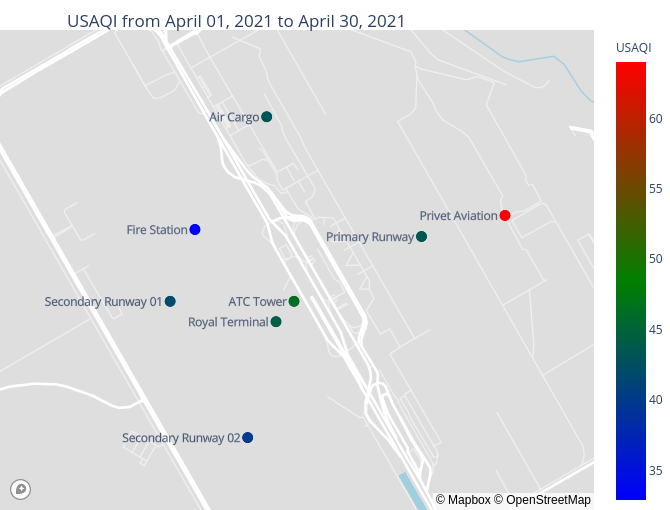
\includegraphics[width=0.90\textwidth]{image22}
\caption{Average AQI per station for \monthyear (1)}\label{image22}
\end{figure}}

\IfFileExists{image23.png}
{\begin{figure}[H]
\centering
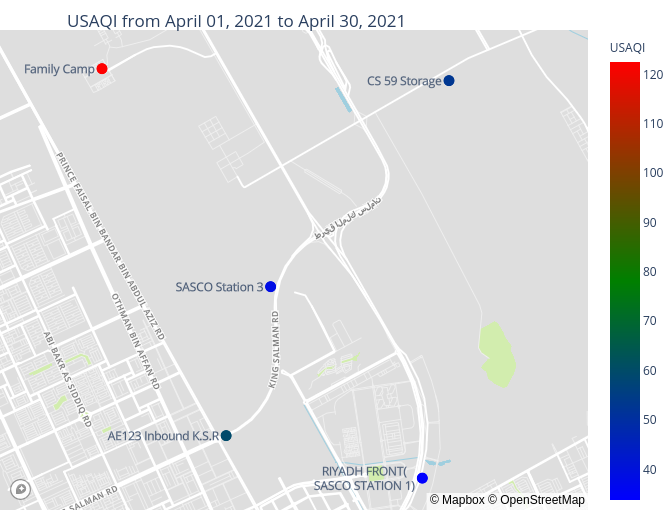
\includegraphics[width=0.90\textwidth]{image23}
\caption{Average AQI per station for \monthyear (2)}\label{image23}
\end{figure}}


As it can be observed in the figure above, the highest AQI averages for the studied period can be found in the station \maxStationAQI. Furthermore, the stations \analysisAQI


\chapter{Conclusions}

\begin{itemize}
\item Measurements for the period of \monthyear \ from \fullstations\ stations installed at RUH airport have been registered and shown in this report.
\item The meteorological measurements are also provided for the study period.
\item Near continuous observations of \ce{CO}, \ce{NO2}, \ce{SO2}, \ce{O3}, \ce{PM_{2.5}}, \ce{PM10}, \ce{PM1}, \ce{CO2}, \ce{H2S}, \ce{NO} as well as the noise metrics Leq, Lmax and Lmin have been obtained. 
\item The \ce{CO2} levels did not show any clear correlation to internal or external sources and were mainly stable during the study period.
\item \concLimits during the study period.
\item The USEPA AQI was calculated from its respective registered pollutant levels and shown as well in this report.
\item \concAQI. Regarding the traffic distribution, the highest number of flights happened on average  \trafficPeriod\ with a peak at 10 pm. They took place most often in the direction \maxRunway.  
\item The PM values could be influenced by external sources, like sandstorms, as indicated in previous monthly reports.
\item It is also important to note that in this analysis only aircraft-related sources affecting Air Quality are considered. Other sources present could be the city of Riyadh, situated south of the airport, the road traffic and natural sources like the dust and sand transported by the wind.
\item Even though the air quality monitoring provides useful information about pollution levels inside and outside the airport, the measurements can be difficult to interpret due to the complex relationship between emissions and air quality levels. A solution to quantify the relative the contribution of an airport to the measured pollution levels is through modelling. Therefore, in order to validate our assumptions made in this report, modelling is an important addition to understand how the pollutant levels can be affected by the traffic. The noise and emissions modelling complement the measurement analysis and help to understand the measurements obtained by the sensors. 
\item We do not find conclusive evidences of aircraft contributing to big extent to pollution levels, therefore, we do not consider air traffic to be a main source of pollution in the studied area. Modelling can help to obtain the quantification of the contribution of aircraft in pollution and noise in Riyadh Airport.
\end{itemize}


\chapter{Acronyms}

\begin{itemize}[leftmargin=2cm]
\item[AQI:] Air Quality Index 
\item[LAQ:] Local Air Quality
\item[Leq:] Equivalent continuous sound level
\item[Lmax:] Maximum root mean squared measured noise level
\item[Lmin:] Lowest root mean squared measured noise level
\item[NAAQS:] National Ambient Air Quality Standards
\item[PM:] Particulate Matter
\item[USEPA:] United States Environmental Protection Agency
\end{itemize}


\appendix

\chapter{Meteorological graphs}
{
\IfFileExists{image24.png}
{\begin{figure}[H]
\centering
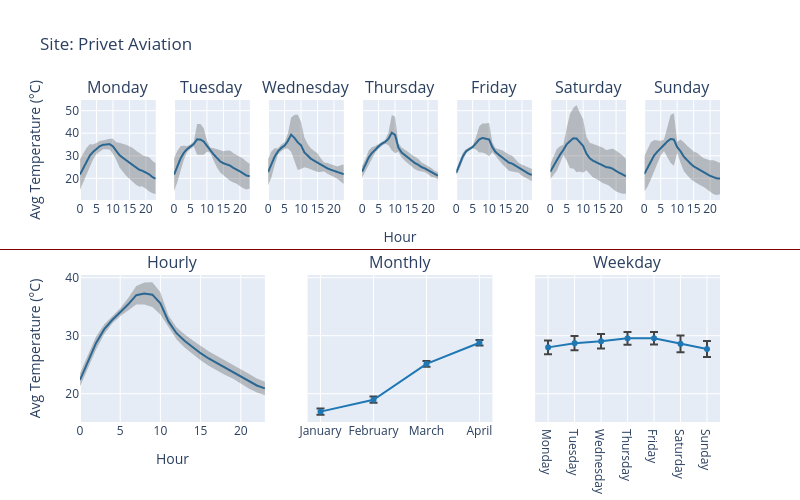
\includegraphics[width=.90\textwidth]{image24}
\end{figure}}{}
\IfFileExists{image25.png}
{\begin{figure}[H]
\centering
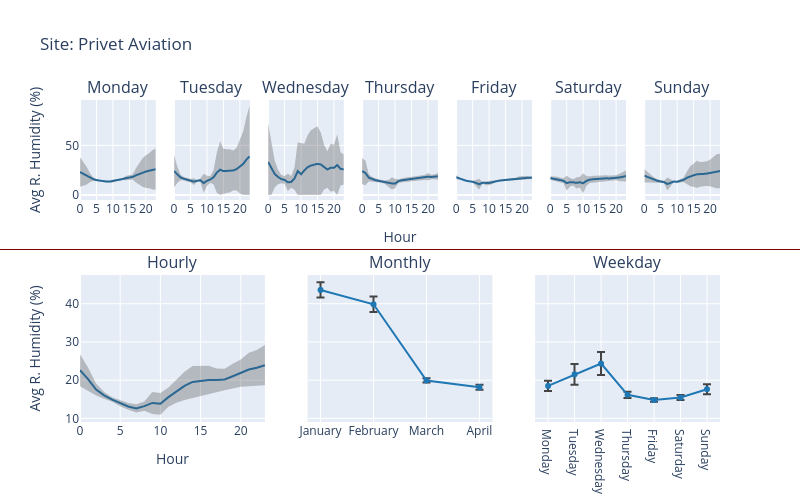
\includegraphics[width=.90\textwidth, keepaspectratio]{image25}
\end{figure}}{}


\chapter{Pollutants charts per station}
\section{AE123 Inbound K.S.R}

\IfFileExists{image26.png} 
{\begin{figure}[H] 
 \centering 
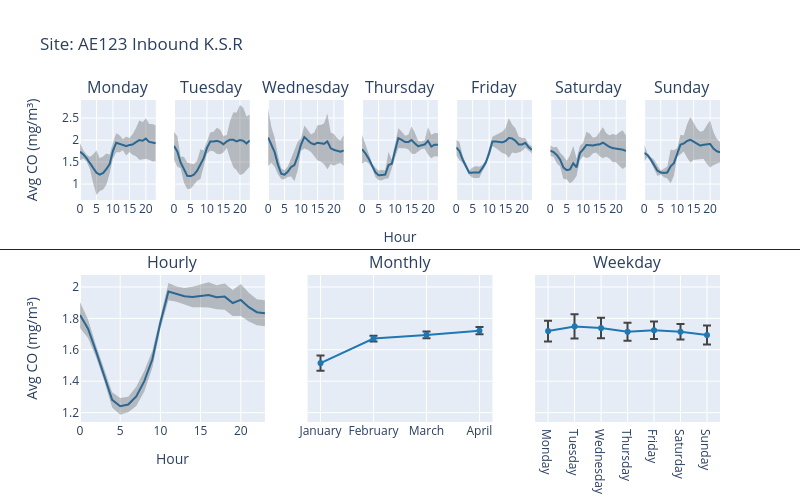
\includegraphics[width=.88\textwidth, keepaspectratio]{image26} 
 \end{figure}}{} 

\IfFileExists{image27.png} 
{\begin{figure}[H] 
 \centering 
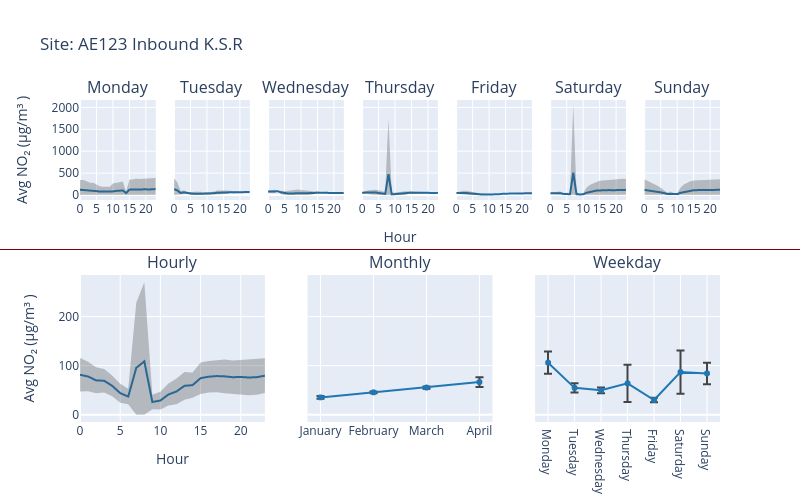
\includegraphics[width=.88\textwidth, keepaspectratio]{image27} 
 \end{figure}}{} 

\IfFileExists{image28.png} 
{\begin{figure}[H] 
 \centering 
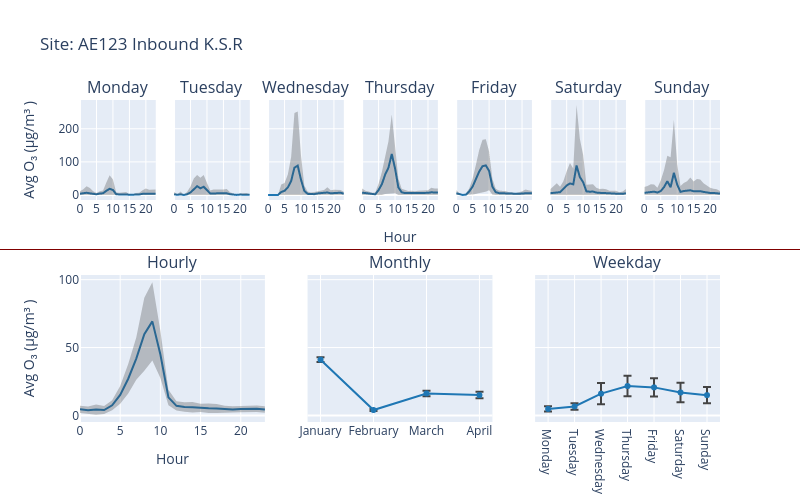
\includegraphics[width=.88\textwidth, keepaspectratio]{image28} 
 \end{figure}}{} 

\IfFileExists{image29.png} 
{\begin{figure}[H] 
 \centering 
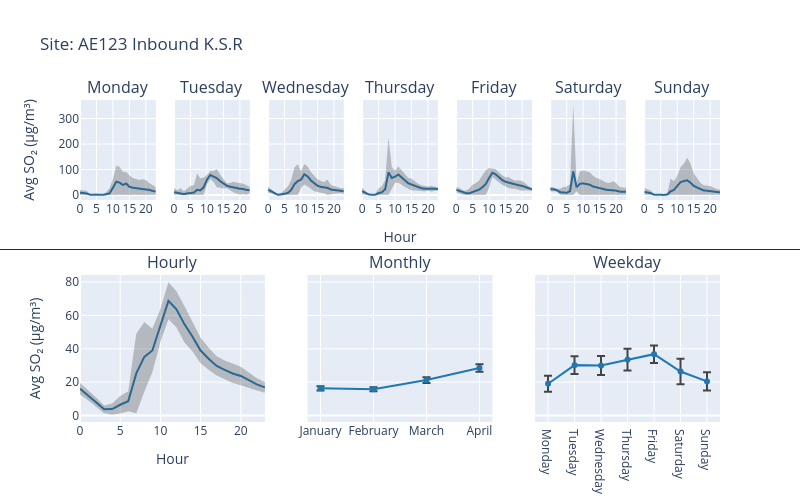
\includegraphics[width=.88\textwidth, keepaspectratio]{image29} 
 \end{figure}}{} 

\IfFileExists{image30.png} 
{\begin{figure}[H] 
 \centering 
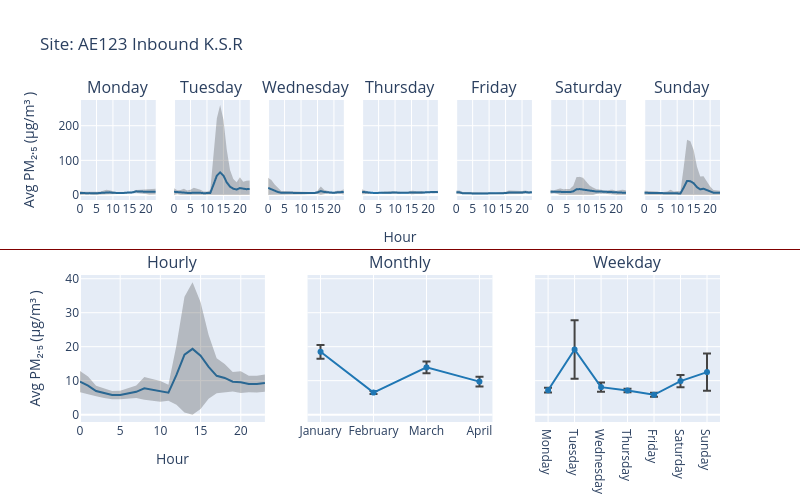
\includegraphics[width=.88\textwidth, keepaspectratio]{image30} 
 \end{figure}}{} 

\IfFileExists{image31.png} 
{\begin{figure}[H] 
 \centering 
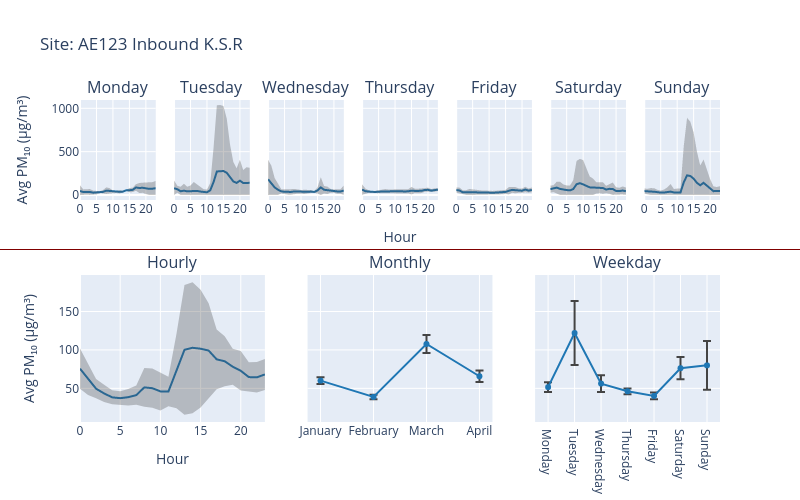
\includegraphics[width=.88\textwidth, keepaspectratio]{image31} 
 \end{figure}}{} 

\IfFileExists{image32.png} 
{\begin{figure}[H] 
 \centering 
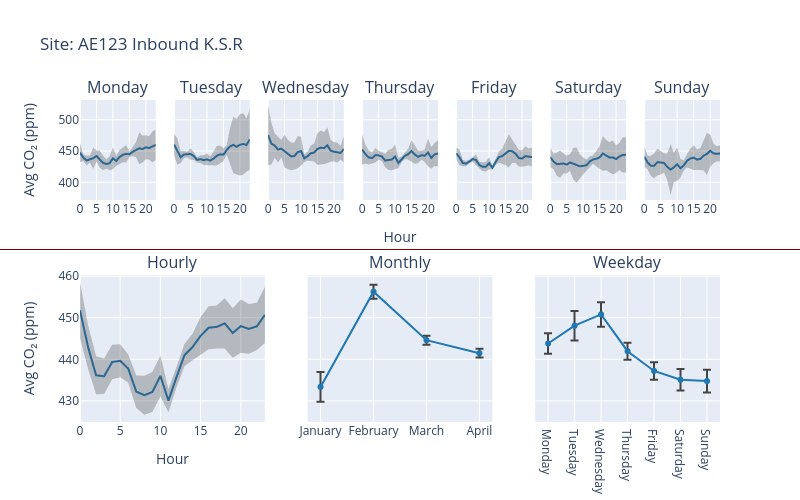
\includegraphics[width=.88\textwidth, keepaspectratio]{image32} 
 \end{figure}}{} 

\IfFileExists{image33.png} 
{\begin{figure}[H] 
 \centering 
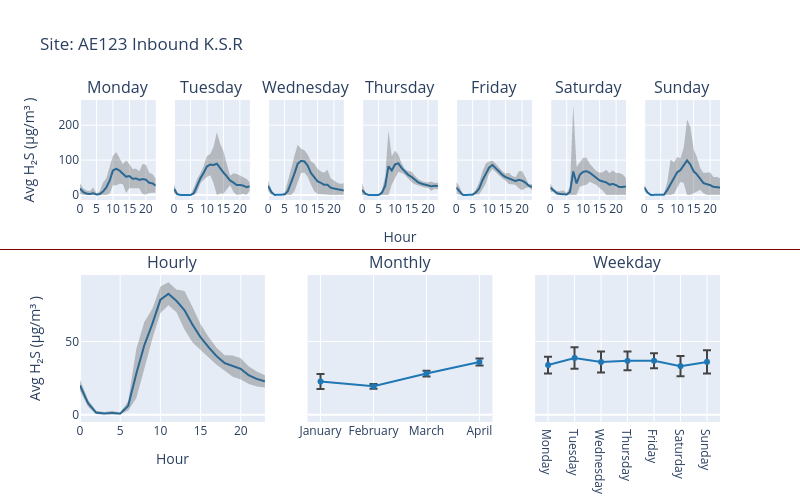
\includegraphics[width=.88\textwidth, keepaspectratio]{image33} 
 \end{figure}}{} 

\IfFileExists{image34.png} 
{\begin{figure}[H] 
 \centering 
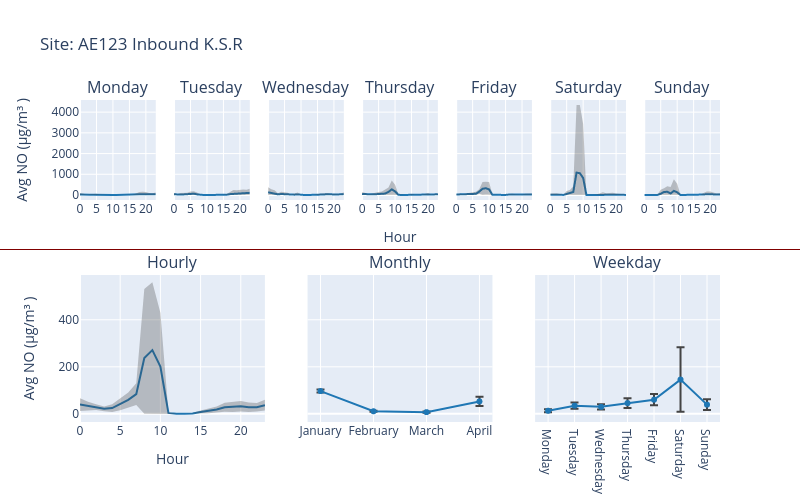
\includegraphics[width=.88\textwidth, keepaspectratio]{image34} 
 \end{figure}}{} 

\IfFileExists{image35.png} 
{\begin{figure}[H] 
 \centering 
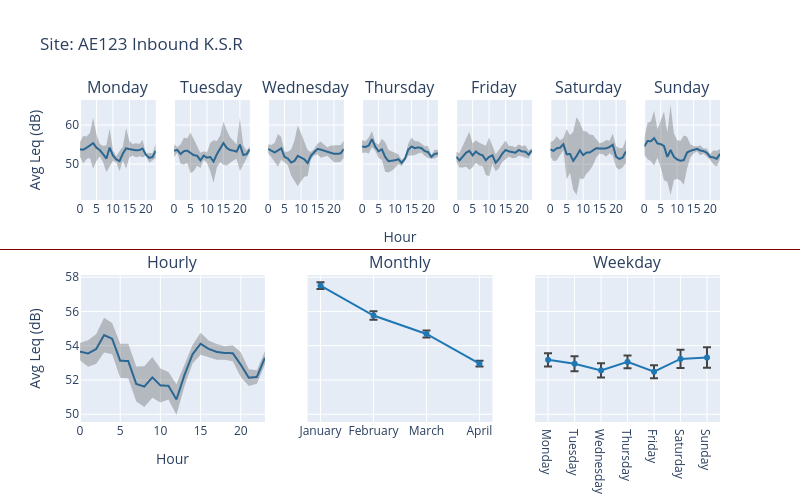
\includegraphics[width=.88\textwidth, keepaspectratio]{image35} 
 \end{figure}}{} 

\IfFileExists{image36.png} 
{\begin{figure}[H] 
 \centering 
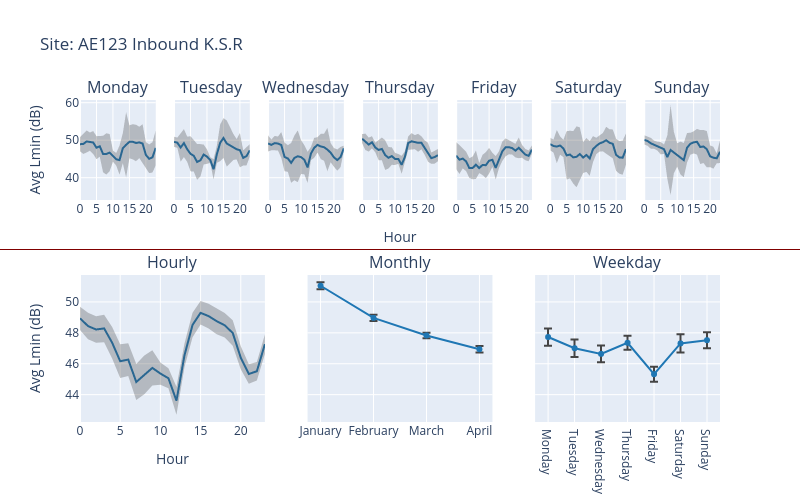
\includegraphics[width=.88\textwidth, keepaspectratio]{image36} 
 \end{figure}}{} 

\IfFileExists{image37.png} 
{\begin{figure}[H] 
 \centering 
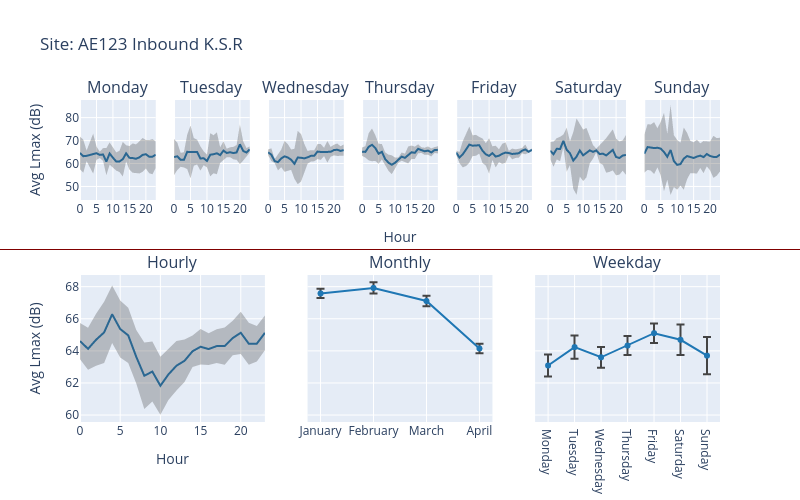
\includegraphics[width=.88\textwidth, keepaspectratio]{image37} 
 \end{figure}}{} 
 

\section{Air Cargo}
\IfFileExists{image38.png} 
{\begin{figure}[H] 
 \centering 
\includegraphics[width=.88\textwidth, keepaspectratio]{image38} 
 \end{figure}}{} 

\IfFileExists{image39.png} 
{\begin{figure}[H] 
 \centering 
\includegraphics[width=.88\textwidth, keepaspectratio]{image39} 
 \end{figure}}{} 

\IfFileExists{image40.png} 
{\begin{figure}[H] 
 \centering 
\includegraphics[width=.88\textwidth, keepaspectratio]{image40} 
 \end{figure}}{} 

\IfFileExists{image41.png} 
{\begin{figure}[H] 
 \centering 
\includegraphics[width=.88\textwidth, keepaspectratio]{image41} 
 \end{figure}}{} 

\IfFileExists{image42.png} 
{\begin{figure}[H] 
 \centering 
\includegraphics[width=.88\textwidth, keepaspectratio]{image42} 
 \end{figure}}{} 

\IfFileExists{image43.png} 
{\begin{figure}[H] 
 \centering 
\includegraphics[width=.88\textwidth, keepaspectratio]{image43} 
 \end{figure}}{} 

\IfFileExists{image44.png} 
{\begin{figure}[H] 
 \centering 
\includegraphics[width=.88\textwidth, keepaspectratio]{image44} 
 \end{figure}}{} 

\IfFileExists{image45.png} 
{\begin{figure}[H] 
 \centering 
\includegraphics[width=.88\textwidth, keepaspectratio]{image45} 
 \end{figure}}{} 

\IfFileExists{image46.png} 
{\begin{figure}[H] 
 \centering 
\includegraphics[width=.88\textwidth, keepaspectratio]{image46} 
 \end{figure}}{} 

\IfFileExists{image47.png} 
{\begin{figure}[H] 
 \centering 
\includegraphics[width=.88\textwidth, keepaspectratio]{image47} 
 \end{figure}}{} 

\IfFileExists{image48.png} 
{\begin{figure}[H] 
 \centering 
\includegraphics[width=.88\textwidth, keepaspectratio]{image48} 
 \end{figure}}{} 

\IfFileExists{image49.png} 
{\begin{figure}[H] 
 \centering 
\includegraphics[width=.88\textwidth, keepaspectratio]{image49} 
 \end{figure}}{} 

\section{ATC Tower}
\IfFileExists{image50.png} 
{\begin{figure}[H] 
 \centering 
\includegraphics[width=.88\textwidth, keepaspectratio]{image50} 
 \end{figure}}{} 

\IfFileExists{image51.png} 
{\begin{figure}[H] 
 \centering 
\includegraphics[width=.88\textwidth, keepaspectratio]{image51} 
 \end{figure}}{} 

\IfFileExists{image52.png} 
{\begin{figure}[H] 
 \centering 
\includegraphics[width=.88\textwidth, keepaspectratio]{image52} 
 \end{figure}}{} 

\IfFileExists{image53.png} 
{\begin{figure}[H] 
 \centering 
\includegraphics[width=.88\textwidth, keepaspectratio]{image53} 
 \end{figure}}{} 

\IfFileExists{image54.png} 
{\begin{figure}[H] 
 \centering 
\includegraphics[width=.88\textwidth, keepaspectratio]{image54} 
 \end{figure}}{} 

\IfFileExists{image55.png} 
{\begin{figure}[H] 
 \centering 
\includegraphics[width=.88\textwidth, keepaspectratio]{image55} 
 \end{figure}}{} 

\IfFileExists{image56.png} 
{\begin{figure}[H] 
 \centering 
\includegraphics[width=.88\textwidth, keepaspectratio]{image56} 
 \end{figure}}{} 

\IfFileExists{image57.png} 
{\begin{figure}[H] 
 \centering 
\includegraphics[width=.88\textwidth, keepaspectratio]{image57} 
 \end{figure}}{} 

\IfFileExists{image58.png} 
{\begin{figure}[H] 
 \centering 
\includegraphics[width=.88\textwidth, keepaspectratio]{image58} 
 \end{figure}}{} 

\IfFileExists{image59.png} 
{\begin{figure}[H] 
 \centering 
\includegraphics[width=.88\textwidth, keepaspectratio]{image59} 
 \end{figure}}{} 

\IfFileExists{image60.png} 
{\begin{figure}[H] 
 \centering 
\includegraphics[width=.88\textwidth, keepaspectratio]{image60} 
 \end{figure}}{} 

\IfFileExists{image61.png} 
{\begin{figure}[H] 
 \centering 
\includegraphics[width=.88\textwidth, keepaspectratio]{image61} 
 \end{figure}}{} 


\section{CS 59 Storage}
\IfFileExists{image62.png} 
{\begin{figure}[H] 
 \centering 
\includegraphics[width=.88\textwidth, keepaspectratio]{image62} 
 \end{figure}}{} 

\IfFileExists{image63.png} 
{\begin{figure}[H] 
 \centering 
\includegraphics[width=.88\textwidth, keepaspectratio]{image63} 
 \end{figure}}{} 

\IfFileExists{image64.png} 
{\begin{figure}[H] 
 \centering 
\includegraphics[width=.88\textwidth, keepaspectratio]{image64} 
 \end{figure}}{} 

\IfFileExists{image65.png} 
{\begin{figure}[H] 
 \centering 
\includegraphics[width=.88\textwidth, keepaspectratio]{image65} 
 \end{figure}}{} 

\IfFileExists{image66.png} 
{\begin{figure}[H] 
 \centering 
\includegraphics[width=.88\textwidth, keepaspectratio]{image66} 
 \end{figure}}{} 

\IfFileExists{image67.png} 
{\begin{figure}[H] 
 \centering 
\includegraphics[width=.88\textwidth, keepaspectratio]{image67} 
 \end{figure}}{} 

\IfFileExists{image68.png} 
{\begin{figure}[H] 
 \centering 
\includegraphics[width=.88\textwidth, keepaspectratio]{image68} 
 \end{figure}}{} 

\IfFileExists{image69.png} 
{\begin{figure}[H] 
 \centering 
\includegraphics[width=.88\textwidth, keepaspectratio]{image69} 
 \end{figure}}{} 

\IfFileExists{image70.png} 
{\begin{figure}[H] 
 \centering 
\includegraphics[width=.88\textwidth, keepaspectratio]{image70} 
 \end{figure}}{} 

\IfFileExists{image71.png} 
{\begin{figure}[H] 
 \centering 
\includegraphics[width=.88\textwidth, keepaspectratio]{image71} 
 \end{figure}}{} 

\IfFileExists{image72.png} 
{\begin{figure}[H] 
 \centering 
\includegraphics[width=.88\textwidth, keepaspectratio]{image72} 
 \end{figure}}{} 

\IfFileExists{image73.png} 
{\begin{figure}[H] 
 \centering 
\includegraphics[width=.88\textwidth, keepaspectratio]{image73} 
 \end{figure}}{} 

\section{Family Camp}
\IfFileExists{image74.png} 
{\begin{figure}[H] 
 \centering 
\includegraphics[width=.88\textwidth, keepaspectratio]{image74} 
 \end{figure}}{} 

\IfFileExists{image75.png} 
{\begin{figure}[H] 
 \centering 
\includegraphics[width=.88\textwidth, keepaspectratio]{image75} 
 \end{figure}}{} 

\IfFileExists{image76.png} 
{\begin{figure}[H] 
 \centering 
\includegraphics[width=.88\textwidth, keepaspectratio]{image76} 
 \end{figure}}{} 

\IfFileExists{image77.png} 
{\begin{figure}[H] 
 \centering 
\includegraphics[width=.88\textwidth, keepaspectratio]{image77} 
 \end{figure}}{} 

\IfFileExists{image78.png} 
{\begin{figure}[H] 
 \centering 
\includegraphics[width=.88\textwidth, keepaspectratio]{image78} 
 \end{figure}}{} 

\IfFileExists{image79.png} 
{\begin{figure}[H] 
 \centering 
\includegraphics[width=.88\textwidth, keepaspectratio]{image79} 
 \end{figure}}{} 

\IfFileExists{image80.png} 
{\begin{figure}[H] 
 \centering 
\includegraphics[width=.88\textwidth, keepaspectratio]{image80} 
 \end{figure}}{} 

\IfFileExists{image81.png} 
{\begin{figure}[H] 
 \centering 
\includegraphics[width=.88\textwidth, keepaspectratio]{image81} 
 \end{figure}}{} 

\IfFileExists{image82.png} 
{\begin{figure}[H] 
 \centering 
\includegraphics[width=.88\textwidth, keepaspectratio]{image82} 
 \end{figure}}{} 

\IfFileExists{image83.png} 
{\begin{figure}[H] 
 \centering 
\includegraphics[width=.88\textwidth, keepaspectratio]{image83} 
 \end{figure}}{} 

\IfFileExists{image84.png} 
{\begin{figure}[H] 
 \centering 
\includegraphics[width=.88\textwidth, keepaspectratio]{image84} 
 \end{figure}}{} 

\IfFileExists{image85.png} 
{\begin{figure}[H] 
 \centering 
\includegraphics[width=.88\textwidth, keepaspectratio]{image85} 
 \end{figure}}{} 

\section{Fire Station}
\IfFileExists{image86.png} 
{\begin{figure}[H] 
 \centering 
\includegraphics[width=.88\textwidth, keepaspectratio]{image86} 
 \end{figure}}{} 

\IfFileExists{image87.png} 
{\begin{figure}[H] 
 \centering 
\includegraphics[width=.88\textwidth, keepaspectratio]{image87} 
 \end{figure}}{} 

\IfFileExists{image88.png} 
{\begin{figure}[H] 
 \centering 
\includegraphics[width=.88\textwidth, keepaspectratio]{image88} 
 \end{figure}}{} 

\IfFileExists{image89.png} 
{\begin{figure}[H] 
 \centering 
\includegraphics[width=.88\textwidth, keepaspectratio]{image89} 
 \end{figure}}{} 

\IfFileExists{image90.png} 
{\begin{figure}[H] 
 \centering 
\includegraphics[width=.88\textwidth, keepaspectratio]{image90} 
 \end{figure}}{} 

\IfFileExists{image91.png} 
{\begin{figure}[H] 
 \centering 
\includegraphics[width=.88\textwidth, keepaspectratio]{image91} 
 \end{figure}}{} 

\IfFileExists{image92.png} 
{\begin{figure}[H] 
 \centering 
\includegraphics[width=.88\textwidth, keepaspectratio]{image92} 
 \end{figure}}{} 

\IfFileExists{image93.png} 
{\begin{figure}[H] 
 \centering 
\includegraphics[width=.88\textwidth, keepaspectratio]{image93} 
 \end{figure}}{} 

\IfFileExists{image94.png} 
{\begin{figure}[H] 
 \centering 
\includegraphics[width=.88\textwidth, keepaspectratio]{image94} 
 \end{figure}}{} 

\IfFileExists{image95.png} 
{\begin{figure}[H] 
 \centering 
\includegraphics[width=.88\textwidth, keepaspectratio]{image95} 
 \end{figure}}{} 

\IfFileExists{image96.png} 
{\begin{figure}[H] 
 \centering 
\includegraphics[width=.88\textwidth, keepaspectratio]{image96} 
 \end{figure}}{} 

\IfFileExists{image97.png} 
{\begin{figure}[H] 
 \centering 
\includegraphics[width=.88\textwidth, keepaspectratio]{image97} 
 \end{figure}}{} 

\section{Primary Runway}
\IfFileExists{image98.png} 
{\begin{figure}[H] 
 \centering 
\includegraphics[width=.88\textwidth, keepaspectratio]{image98} 
 \end{figure}}{} 

\IfFileExists{image99.png} 
{\begin{figure}[H] 
 \centering 
\includegraphics[width=.88\textwidth, keepaspectratio]{image99} 
 \end{figure}}{} 

\IfFileExists{image100.png} 
{\begin{figure}[H] 
 \centering 
\includegraphics[width=.88\textwidth, keepaspectratio]{image100} 
 \end{figure}}{} 

\IfFileExists{image101.png} 
{\begin{figure}[H] 
 \centering 
\includegraphics[width=.88\textwidth, keepaspectratio]{image101} 
 \end{figure}}{} 

\IfFileExists{image102.png} 
{\begin{figure}[H] 
 \centering 
\includegraphics[width=.88\textwidth, keepaspectratio]{image102} 
 \end{figure}}{} 

\IfFileExists{image103.png} 
{\begin{figure}[H] 
 \centering 
\includegraphics[width=.88\textwidth, keepaspectratio]{image103} 
 \end{figure}}{} 

\IfFileExists{image104.png} 
{\begin{figure}[H] 
 \centering 
\includegraphics[width=.88\textwidth, keepaspectratio]{image104} 
 \end{figure}}{} 

\IfFileExists{image105.png} 
{\begin{figure}[H] 
 \centering 
\includegraphics[width=.88\textwidth, keepaspectratio]{image105} 
 \end{figure}}{} 

\IfFileExists{image106.png} 
{\begin{figure}[H] 
 \centering 
\includegraphics[width=.88\textwidth, keepaspectratio]{image106} 
 \end{figure}}{} 

\IfFileExists{image107.png} 
{\begin{figure}[H] 
 \centering 
\includegraphics[width=.88\textwidth, keepaspectratio]{image107} 
 \end{figure}}{} 

\IfFileExists{image108.png} 
{\begin{figure}[H] 
 \centering 
\includegraphics[width=.88\textwidth, keepaspectratio]{image108} 
 \end{figure}}{} 

\IfFileExists{image109.png} 
{\begin{figure}[H] 
 \centering 
\includegraphics[width=.88\textwidth, keepaspectratio]{image109} 
 \end{figure}}{} 

\section{Privet Aviation}
\IfFileExists{image110.png} 
{\begin{figure}[H] 
 \centering 
\includegraphics[width=.88\textwidth, keepaspectratio]{image110} 
 \end{figure}}{} 

\IfFileExists{image111.png} 
{\begin{figure}[H] 
 \centering 
\includegraphics[width=.88\textwidth, keepaspectratio]{image111} 
 \end{figure}}{} 

\IfFileExists{image112.png} 
{\begin{figure}[H] 
 \centering 
\includegraphics[width=.88\textwidth, keepaspectratio]{image112} 
 \end{figure}}{} 

\IfFileExists{image113.png} 
{\begin{figure}[H] 
 \centering 
\includegraphics[width=.88\textwidth, keepaspectratio]{image113} 
 \end{figure}}{} 

\IfFileExists{image114.png} 
{\begin{figure}[H] 
 \centering 
\includegraphics[width=.88\textwidth, keepaspectratio]{image114} 
 \end{figure}}{} 

\IfFileExists{image115.png} 
{\begin{figure}[H] 
 \centering 
\includegraphics[width=.88\textwidth, keepaspectratio]{image115} 
 \end{figure}}{} 

\IfFileExists{image116.png} 
{\begin{figure}[H] 
 \centering 
\includegraphics[width=.88\textwidth, keepaspectratio]{image116} 
 \end{figure}}{} 

\IfFileExists{image117.png} 
{\begin{figure}[H] 
 \centering 
\includegraphics[width=.88\textwidth, keepaspectratio]{image117} 
 \end{figure}}{} 

\IfFileExists{image118.png} 
{\begin{figure}[H] 
 \centering 
\includegraphics[width=.88\textwidth, keepaspectratio]{image118} 
 \end{figure}}{} 

\IfFileExists{image119.png} 
{\begin{figure}[H] 
 \centering 
\includegraphics[width=.88\textwidth, keepaspectratio]{image119} 
 \end{figure}}{} 

\IfFileExists{image120.png} 
{\begin{figure}[H] 
 \centering 
\includegraphics[width=.88\textwidth, keepaspectratio]{image120} 
 \end{figure}}{} 

\IfFileExists{image121.png} 
{\begin{figure}[H] 
 \centering 
\includegraphics[width=.88\textwidth, keepaspectratio]{image121} 
 \end{figure}}{} 

\section{RIYADH FRONT (SASCO STATION 1)}
\IfFileExists{image122.png} 
{\begin{figure}[H] 
 \centering 
\includegraphics[width=.88\textwidth, keepaspectratio]{image122} 
 \end{figure}}{} 

\IfFileExists{image123.png} 
{\begin{figure}[H] 
 \centering 
\includegraphics[width=.88\textwidth, keepaspectratio]{image123} 
 \end{figure}}{} 

\IfFileExists{image124.png} 
{\begin{figure}[H] 
 \centering 
\includegraphics[width=.88\textwidth, keepaspectratio]{image124} 
 \end{figure}}{} 

\IfFileExists{image125.png} 
{\begin{figure}[H] 
 \centering 
\includegraphics[width=.88\textwidth, keepaspectratio]{image125} 
 \end{figure}}{} 

\IfFileExists{image126.png} 
{\begin{figure}[H] 
 \centering 
\includegraphics[width=.88\textwidth, keepaspectratio]{image126} 
 \end{figure}}{} 

\IfFileExists{image127.png} 
{\begin{figure}[H] 
 \centering 
\includegraphics[width=.88\textwidth, keepaspectratio]{image127} 
 \end{figure}}{} 

\IfFileExists{image128.png} 
{\begin{figure}[H] 
 \centering 
\includegraphics[width=.88\textwidth, keepaspectratio]{image128} 
 \end{figure}}{} 

\IfFileExists{image129.png} 
{\begin{figure}[H] 
 \centering 
\includegraphics[width=.88\textwidth, keepaspectratio]{image129} 
 \end{figure}}{} 

\IfFileExists{image130.png} 
{\begin{figure}[H] 
 \centering 
\includegraphics[width=.88\textwidth, keepaspectratio]{image130} 
 \end{figure}}{} 

\IfFileExists{image131.png} 
{\begin{figure}[H] 
 \centering 
\includegraphics[width=.88\textwidth, keepaspectratio]{image131} 
 \end{figure}}{} 

\IfFileExists{image132.png} 
{\begin{figure}[H] 
 \centering 
\includegraphics[width=.88\textwidth, keepaspectratio]{image132} 
 \end{figure}}{} 

\IfFileExists{image133.png} 
{\begin{figure}[H] 
 \centering 
\includegraphics[width=.88\textwidth, keepaspectratio]{image133} 
 \end{figure}}{} 


\section{Royal Terminal}
\IfFileExists{image134.png} 
{\begin{figure}[H] 
 \centering 
\includegraphics[width=.88\textwidth, keepaspectratio]{image134} 
 \end{figure}}{} 

\IfFileExists{image135.png} 
{\begin{figure}[H] 
 \centering 
\includegraphics[width=.88\textwidth, keepaspectratio]{image135} 
 \end{figure}}{} 

\IfFileExists{image136.png} 
{\begin{figure}[H] 
 \centering 
\includegraphics[width=.88\textwidth, keepaspectratio]{image136} 
 \end{figure}}{} 

\IfFileExists{image137.png} 
{\begin{figure}[H] 
 \centering 
\includegraphics[width=.88\textwidth, keepaspectratio]{image137} 
 \end{figure}}{} 

\IfFileExists{image138.png} 
{\begin{figure}[H] 
 \centering 
\includegraphics[width=.88\textwidth, keepaspectratio]{image138} 
 \end{figure}}{} 

\IfFileExists{image139.png} 
{\begin{figure}[H] 
 \centering 
\includegraphics[width=.88\textwidth, keepaspectratio]{image139} 
 \end{figure}}{} 

\IfFileExists{image140.png} 
{\begin{figure}[H] 
 \centering 
\includegraphics[width=.88\textwidth, keepaspectratio]{image140} 
 \end{figure}}{} 

\IfFileExists{image141.png} 
{\begin{figure}[H] 
 \centering 
\includegraphics[width=.88\textwidth, keepaspectratio]{image141} 
 \end{figure}}{} 

\IfFileExists{image142.png} 
{\begin{figure}[H] 
 \centering 
\includegraphics[width=.88\textwidth, keepaspectratio]{image142} 
 \end{figure}}{} 

\IfFileExists{image143.png} 
{\begin{figure}[H] 
 \centering 
\includegraphics[width=.88\textwidth, keepaspectratio]{image143} 
 \end{figure}}{} 

\IfFileExists{image144.png} 
{\begin{figure}[H] 
 \centering 
\includegraphics[width=.88\textwidth, keepaspectratio]{image144} 
 \end{figure}}{} 

\IfFileExists{image145.png} 
{\begin{figure}[H] 
 \centering 
\includegraphics[width=.88\textwidth, keepaspectratio]{image145} 
 \end{figure}}{} 

\section{SASCO Station 3}
\IfFileExists{image146.png} 
{\begin{figure}[H] 
 \centering 
\includegraphics[width=.88\textwidth, keepaspectratio]{image146} 
 \end{figure}}{} 

\IfFileExists{image147.png} 
{\begin{figure}[H] 
 \centering 
\includegraphics[width=.88\textwidth, keepaspectratio]{image147} 
 \end{figure}}{} 

\IfFileExists{image148.png} 
{\begin{figure}[H] 
 \centering 
\includegraphics[width=.88\textwidth, keepaspectratio]{image148} 
 \end{figure}}{} 

\IfFileExists{image149.png} 
{\begin{figure}[H] 
 \centering 
\includegraphics[width=.88\textwidth, keepaspectratio]{image149} 
 \end{figure}}{} 

\IfFileExists{image150.png} 
{\begin{figure}[H] 
 \centering 
\includegraphics[width=.88\textwidth, keepaspectratio]{image150} 
 \end{figure}}{} 

\IfFileExists{image151.png} 
{\begin{figure}[H] 
 \centering 
\includegraphics[width=.88\textwidth, keepaspectratio]{image151} 
 \end{figure}}{} 

\IfFileExists{image152.png} 
{\begin{figure}[H] 
 \centering 
\includegraphics[width=.88\textwidth, keepaspectratio]{image152} 
 \end{figure}}{} 

\IfFileExists{image153.png} 
{\begin{figure}[H] 
 \centering 
\includegraphics[width=.88\textwidth, keepaspectratio]{image153} 
 \end{figure}}{} 

\IfFileExists{image154.png} 
{\begin{figure}[H] 
 \centering 
\includegraphics[width=.88\textwidth, keepaspectratio]{image154} 
 \end{figure}}{} 

\IfFileExists{image155.png} 
{\begin{figure}[H] 
 \centering 
\includegraphics[width=.88\textwidth, keepaspectratio]{image155} 
 \end{figure}}{} 

\IfFileExists{image156.png} 
{\begin{figure}[H] 
 \centering 
\includegraphics[width=.88\textwidth, keepaspectratio]{image156} 
 \end{figure}}{} 

\IfFileExists{image157.png} 
{\begin{figure}[H] 
 \centering 
\includegraphics[width=.88\textwidth, keepaspectratio]{image157} 
 \end{figure}}{} 

\section{ Secondary Runway 01}
\IfFileExists{image158.png} 
{\begin{figure}[H] 
 \centering 
\includegraphics[width=.88\textwidth, keepaspectratio]{image158} 
 \end{figure}}{} 

\IfFileExists{image159.png} 
{\begin{figure}[H] 
 \centering 
\includegraphics[width=.88\textwidth, keepaspectratio]{image159} 
 \end{figure}}{} 

\IfFileExists{image160.png} 
{\begin{figure}[H] 
 \centering 
\includegraphics[width=.88\textwidth, keepaspectratio]{image160} 
 \end{figure}}{} 

\IfFileExists{image161.png} 
{\begin{figure}[H] 
 \centering 
\includegraphics[width=.88\textwidth, keepaspectratio]{image161} 
 \end{figure}}{} 

\IfFileExists{image162.png} 
{\begin{figure}[H] 
 \centering 
\includegraphics[width=.88\textwidth, keepaspectratio]{image162} 
 \end{figure}}{} 

\IfFileExists{image163.png} 
{\begin{figure}[H] 
 \centering 
\includegraphics[width=.88\textwidth, keepaspectratio]{image163} 
 \end{figure}}{} 

\IfFileExists{image164.png} 
{\begin{figure}[H] 
 \centering 
\includegraphics[width=.88\textwidth, keepaspectratio]{image164} 
 \end{figure}}{} 

\IfFileExists{image165.png} 
{\begin{figure}[H] 
 \centering 
\includegraphics[width=.88\textwidth, keepaspectratio]{image165} 
 \end{figure}}{} 

\IfFileExists{image166.png} 
{\begin{figure}[H] 
 \centering 
\includegraphics[width=.88\textwidth, keepaspectratio]{image166} 
 \end{figure}}{} 

\IfFileExists{image167.png} 
{\begin{figure}[H] 
 \centering 
\includegraphics[width=.88\textwidth, keepaspectratio]{image167} 
 \end{figure}}{} 

\IfFileExists{image168.png} 
{\begin{figure}[H] 
 \centering 
\includegraphics[width=.88\textwidth, keepaspectratio]{image168} 
 \end{figure}}{} 

\IfFileExists{image169.png} 
{\begin{figure}[H] 
 \centering 
\includegraphics[width=.88\textwidth, keepaspectratio]{image169} 
 \end{figure}}{} 

\section{Secondary Runway 02}
\IfFileExists{image170.png} 
{\begin{figure}[H] 
 \centering 
\includegraphics[width=.88\textwidth, keepaspectratio]{image170} 
 \end{figure}}{} 

\IfFileExists{image171.png} 
{\begin{figure}[H] 
 \centering 
\includegraphics[width=.88\textwidth, keepaspectratio]{image171} 
 \end{figure}}{} 

\IfFileExists{image172.png} 
{\begin{figure}[H] 
 \centering 
\includegraphics[width=.88\textwidth, keepaspectratio]{image172} 
 \end{figure}}{} 

\IfFileExists{image173.png} 
{\begin{figure}[H] 
 \centering 
\includegraphics[width=.88\textwidth, keepaspectratio]{image173} 
 \end{figure}}{} 

\IfFileExists{image174.png} 
{\begin{figure}[H] 
 \centering 
\includegraphics[width=.88\textwidth, keepaspectratio]{image174} 
 \end{figure}}{} 

\IfFileExists{image175.png} 
{\begin{figure}[H] 
 \centering 
\includegraphics[width=.88\textwidth, keepaspectratio]{image175} 
 \end{figure}}{} 

\IfFileExists{image176.png} 
{\begin{figure}[H] 
 \centering 
\includegraphics[width=.88\textwidth, keepaspectratio]{image176} 
 \end{figure}}{} 

\IfFileExists{image177.png} 
{\begin{figure}[H] 
 \centering 
\includegraphics[width=.88\textwidth, keepaspectratio]{image177} 
 \end{figure}}{} 

\IfFileExists{image178.png} 
{\begin{figure}[H] 
 \centering 
\includegraphics[width=.88\textwidth, keepaspectratio]{image178} 
 \end{figure}}{} 

\IfFileExists{image179.png} 
{\begin{figure}[H] 
 \centering 
\includegraphics[width=.88\textwidth, keepaspectratio]{image179} 
 \end{figure}}{} 

\IfFileExists{image180.png} 
{\begin{figure}[H] 
 \centering 
\includegraphics[width=.88\textwidth, keepaspectratio]{image180} 
 \end{figure}}{} 

\IfFileExists{image181.png} 
{\begin{figure}[H] 
 \centering 
\includegraphics[width=.88\textwidth, keepaspectratio]{image181} 
 \end{figure}}{} 




\chapter{Traffic chart}

\IfFileExists{traffic.png}
{\begin{figure}[H]
\centering
\includegraphics[width=1\textwidth, keepaspectratio]{traffic}
\end{figure}}{}


\chapter{Monthly grouped charts}
\IfFileExists{image182.png}
{\begin{figure}[H]
\centering
\includegraphics[width=\textwidth]{image182}
\caption{One-hour average \ce{CO} concentrations 1}\label{image182}
\end{figure}}{}

\IfFileExists{image194.png}
{\begin{figure}[H]
\centering
\includegraphics[width=\textwidth]{image194}
\caption{One-hour average \ce{CO} concentrations 2}\label{image194}
\end{figure}}{}


\IfFileExists{image206.png}
{\begin{figure}[H]
\centering
\includegraphics[width=\textwidth]{image206}
\caption{One-hour average \ce{CO} concentrations 3}\label{image206}
\end{figure}}{}

\IfFileExists{image218.png}
{\begin{figure}[H]
\centering
\includegraphics[width=\textwidth]{image218}
\caption{One-hour average \ce{CO} concentrations 4}\label{image218}
\end{figure}}{}

\IfFileExists{image183.png}
{\begin{figure}[H]
\centering
\includegraphics[width=\textwidth]{image183}
\caption{One-hour average \ce{NO2} concentrations 1}\label{image183}
\end{figure}}{}

\
\IfFileExists{image195.png}
{\begin{figure}[H]
\centering
\includegraphics[width=\textwidth]{image195}
\caption{One-hour average \ce{NO2} concentrations 2}\label{image195}
\end{figure}}{}



\IfFileExists{image207.png}
{\begin{figure}[H]
\centering
\includegraphics[width=\textwidth]{image207}
\caption{One-hour average \ce{NO2} concentrations 3}\label{image207}
\end{figure}}{}


\IfFileExists{image219.png}
{\begin{figure}[H]
\centering
\includegraphics[width=\textwidth]{image219}
\caption{One-hour average \ce{NO2} concentrations 4}\label{image219}
\end{figure}}{}


\IfFileExists{image184.png}
{\begin{figure}[H]
\centering
\includegraphics[width=\textwidth]{image184}
\caption{Eight-hours average \ce{O3} concentrations 1}\label{image184}
\end{figure}}{}


\IfFileExists{image196.png}
{\begin{figure}[H]
\centering
\includegraphics[width=\textwidth]{image196}
\caption{Eight-hours average \ce{O3} concentrations 2}\label{image196}
\end{figure}}{}

\IfFileExists{image208.png}
{\begin{figure}[H]
\centering
\includegraphics[width=\textwidth]{image208}
\caption{Eight-hours average \ce{O3} concentrations 3}\label{image208}
\end{figure}}{}

\IfFileExists{image220.png}
{\begin{figure}[H]
\centering
\includegraphics[width=\textwidth]{image220}
\caption{Eight-hours average \ce{O3} concentrations 4}\label{image220}
\end{figure}}{}

\IfFileExists{image185.png}
{\begin{figure}[H]
\centering
\includegraphics[width=\textwidth]{image185}
\caption{One-hour average \ce{SO2} concentrations 1}\label{image185}
\end{figure}}{}

\IfFileExists{image197.png}
{\begin{figure}[H]
\centering
\includegraphics[width=\textwidth]{image197}
\caption{One-hour average \ce{SO2} concentrations 2}\label{image197}
\end{figure}}{}


\IfFileExists{image209.png}
{\begin{figure}[H]
\centering
\includegraphics[width=\textwidth]{image209}
\caption{One-hour average \ce{SO2} concentrations 3}\label{image209}
\end{figure}}{}

\IfFileExists{image221.png}
{\begin{figure}[H]
\centering
\includegraphics[width=\textwidth]{image221}
\caption{One-hour average \ce{SO2} concentrations 4}\label{image221}
\end{figure}}{}

\IfFileExists{image186.png}
{\begin{figure}[H]
\centering
\includegraphics[width=\textwidth]{image186}
\caption{24-hours average \ce{PM_{2.5}} concentrations 1}\label{image186}
\end{figure}}{}


\IfFileExists{image198.png}
{\begin{figure}[H]
\centering
\includegraphics[width=\textwidth]{image198}
\caption{24-hours average \ce{PM_{2.5}} concentrations 2}\label{image198}
\end{figure}}{}


\IfFileExists{image210.png}
{\begin{figure}[H]
\centering
\includegraphics[width=\textwidth]{image210}
\caption{24-hours average \ce{PM_{2.5}} concentrations 3}\label{image210}
\end{figure}}{}


\IfFileExists{image222.png}
{\begin{figure}[H]
\centering
\includegraphics[width=\textwidth]{image222}
\caption{24-hours average \ce{PM_{2.5}} concentrations 4}\label{image222}
\end{figure}}{}

\IfFileExists{image187.png}
{\begin{figure}[H]
\centering
\includegraphics[width=\textwidth]{image187}
\caption{24-hours average \ce{PM10} concentrations 1}\label{image187}
\end{figure}}{}


\IfFileExists{image199.png}
{\begin{figure}[H]
\centering
\includegraphics[width=\textwidth]{image199}
\caption{24-hours average \ce{PM10} concentrations 2}\label{image199}
\end{figure}}{}


\IfFileExists{image211.png}
{\begin{figure}[H]
\centering
\includegraphics[width=\textwidth]{image211}
\caption{24-hours average \ce{PM10} concentrations 3}\label{image211}
\end{figure}}{}

\IfFileExists{image223.png}
{\begin{figure}[H]
\centering
\includegraphics[width=\textwidth]{image223}
\caption{24-hours average \ce{PM10} concentrations 4}\label{image223}
\end{figure}}{}



\IfFileExists{image188.png}
{\begin{figure}[H]
\centering
\includegraphics[width=\textwidth]{image188}
\caption{One-hour average \ce{CO2} concentrations 1}\label{image188}
\end{figure}}{}

\bigskip
\IfFileExists{image200.png}
{\begin{figure}[H]
\centering
\includegraphics[width=\textwidth]{image200}
\caption{One-hour average \ce{CO2} concentrations 2}\label{image200}
\end{figure}}{}

\IfFileExists{image212.png}
{\begin{figure}[H]
\centering
\includegraphics[width=\textwidth]{image212}
\caption{One-hour average \ce{CO2} concentrations 3}\label{image212}
\end{figure}}{}

\IfFileExists{image224.png}
{\begin{figure}[H]
\centering
\includegraphics[width=\textwidth]{image224}
\caption{One-hour average \ce{CO2} concentrations 4}\label{image224}
\end{figure}}{}


\IfFileExists{image189.png}
{\begin{figure}[H]
\centering
\includegraphics[width=\textwidth]{image189}
\caption{One-hour average \ce{H2S} concentrations 1}\label{image189}
\end{figure}}{}

\bigskip
\IfFileExists{image201.png}
{\begin{figure}[H]
\centering
\includegraphics[width=\textwidth]{image201}
\caption{One-hour average \ce{H2S} concentrations 2}\label{image201}
\end{figure}}{}


\IfFileExists{image213.png}
{\begin{figure}[H]
\centering
\includegraphics[width=\textwidth]{image213}
\caption{One-hour average \ce{H2S} concentrations 3}\label{image213}
\end{figure}}{}


\IfFileExists{image225.png}
{\begin{figure}[H]
\centering
\includegraphics[width=\textwidth]{image225}
\caption{One-hour average \ce{H2S} concentrations 4}\label{image225}
\end{figure}}{}



\IfFileExists{image190.png}
{\begin{figure}[H]
\centering
\includegraphics[width=\textwidth]{image190}
\caption{One-hour average \ce{NO} concentrations 1}\label{image190}
\end{figure}}{}


\IfFileExists{image202.png}
{\begin{figure}[H]
\centering
\includegraphics[width=\textwidth]{image202}
\caption{One-hour average \ce{NO} concentrations 2}\label{image202}
\end{figure}}{}


\IfFileExists{image214.png}
{\begin{figure}[H]
\centering
\includegraphics[width=\textwidth]{image214}
\caption{One-hour average \ce{NO} concentrations 3}\label{image214}
\end{figure}}{}


\IfFileExists{image226.png}
{\begin{figure}[H]
\centering
\includegraphics[width=\textwidth]{image226}
\caption{One-hour average \ce{NO} concentrations 4}\label{image226}
\end{figure}}{}

\newpage

\centering
\vspace*{\fill}
\includegraphics[width=4.5cm]{logo.png}\\[6pt]
{\bfseries\footnotesize
62 rue Montorgueil, BAL 9, \\ 
75002 Paris \\
FRANCE \\[-4pt]
\url{www.env-isa.com}
}

\end{document}
